\documentclass[11pt, a4paper]{report}
%-----------NORSK LaTeX--------------

% Denne pakken inkluderer skandinaviske bokstaver( æ, ø og å)
\usepackage[utf8]{inputenc}

% Denne pakken bruker norsk typesetting (innholdsliste osv.)
\usepackage[norsk]{babel}

%--------DOKUMENTOPPSETT------------

% Lar deg tilpasse layouten i prosjektet
\usepackage{fancyhdr}

% Definere egne farger 
\usepackage[usenames, dvipsnames]{color}

% Avstand på marger til sidene på arket
%\usepackage{geometry}

% Linker i dokumentet (figurer, seksjoner osv)
\usepackage[hidelinks]{hyperref}

% Kildeliste-setup
%\usepackage[natbibapa]{apacite} % For apalike eller apacite
\usepackage{natbib} % For Chicago, Vancover, Harvard Style, Nature Style osv

% Spacing mellom bokstaver
\usepackage{microtype}

% Laster inn forskjellige skrifttyper
\usepackage{uarial} % Arial
\usepackage[scaled]{helvet} % Helvetica
%\usepackage{tgbonum} % Usikker
%\usepackage{mathptmx} % Times New Roman
%\usepackage{lmodern} % Latin Modern
%\usepackage[charter]{mathdesign} % Charters
\usepackage[T1]{fontenc}

% Avsnitt mellom paragrafer
\usepackage{parskip}

% Linjeavstand i dokumentet
\usepackage{setspace}
\setlength{\parskip}{1em}

% Fet skrift på alle figurnr
\usepackage[labelfont=bf]{caption}
\usepackage{capt-of}
\usepackage{caption}

\usepackage{chngcntr}
\counterwithin{figure}{chapter}
\counterwithin{table}{chapter}

% Definerer mellomrom mellom seksjons-, figur- og tabellnummer i innholdsliste til teksten begynner
\renewcommand{\numberline}[1]{#1 \,}

% Kan skrive i kolonner
\usepackage{multicol}

% For appendix
\usepackage{titletoc}
\usepackage{appendix}

%----------ANDRE PAKKER--------------

% Pakker fra AMS. Kan skrive matteformler
\usepackage{amsfonts, amssymb, amsthm}
\usepackage{mathtools}

% For grafikk (lime inn bilder, pdf-dokumenter)
\usepackage{graphicx}
\usepackage{float}
\usepackage{pdfpages}
\usepackage{subcaption}

% For inportering av csv-filer som tabeller. ( Ikkje i bruk)
%usepackage{csvsimple}

% Pakke for citations
%\usepackage{biblatex}
% Pakke for at url linker skal fungere i bl.a. referansar
\usepackage{url}

% Generere tekst
\usepackage{kantlipsum}

% Definere egne objekt
\usepackage{tikz}

% Lar deg lage lister på en mer oversiktlig måte
\usepackage[sharp]{easylist}

% Boks rundt tekst
\usepackage{fancyvrb}

% Test pakker
\usepackage{array}
\usepackage[margin=1in]{geometry} % Juster margene etter behov
\usepackage{titlesec}
\usepackage{tabularx}
\usepackage[table]{xcolor}
\usepackage{lastpage}

% pakke for ordliste
\usepackage[automake]{glossaries-extra}

% For å kunne justere bilete
\usepackage{adjustbox}

% 
\usepackage{tocloft}

%---------------------------------------------------

% Velger arial som skrifttype i dokumentet 
%\renewcommand{\rmdefault}{qpl} % 
%\renewcommand{\rmdefault}{phv} % Arial
\renewcommand*\familydefault{\sfdefault} % Helvetica(sans-serif)


% Definerer egne farger
\definecolor{mybla}{RGB}{25, 49, 90}
\definecolor{mylysbla}{RGB}{0, 136, 176}
\definecolor{renasysGreen}{RGB}{4, 255, 4}
\definecolor{purewhite}{RGB}{255,255,255}
\definecolor{lightgray}{gray}{0.8}
\definecolor{myblack}{gray}{0.1}

% Velger norsk språk på innholdsfortegnelse, figurliste, tabelliste og Referanseliste
% Legger disse så til i innholdsfortegnelsen.
\addto\captionsnorsk{\renewcommand{\contentsname}{Innhaldsliste}}
\addto\captionsnorsk{\renewcommand{\listfigurename}{Figurliste}}
\addto\captionsnorsk{\renewcommand{\listtablename}{Tabelliste}}
\addto\captionsnorsk{\renewcommand{\bibname}{Referansar}}
% Nynorsk!
\addto\captionsnynorsk{\renewcommand{\contentsname}{Innhaldsliste}} 
\addto\captionsnynorsk{\renewcommand{\listfigurename}{Figurliste}}
\addto\captionsnynorsk{\renewcommand{\listtablename}{Tabelliste}}
\addto\captionsnynorsk{\renewcommand{\bibname}{Referansar}}


% ----- Justering av avstander mellom chapter / section / subsection / subsubsection

% Justeringa av chapter, 
% første verdi : Horisontalverdi frå venstre marg
% Andre verdi : avstanden frå toppen av sida til tittelen
% Tredje verdi : Avstand til neste tekst
\titleformat{\chapter}[hang]
  {\normalfont\bfseries\LARGE}{\thechapter}{1em}{}
\titlespacing*{\chapter}{0pt}{-50pt}{20pt}

% Juster avstanden for \section
\titleformat{\section}
  {\normalfont\Large\bfseries}{\thesection}{1em}{}
\titlespacing*{\section}{0pt}{10pt}{10pt}

% Juster avstanden for \subsection
\titleformat{\subsection}
  {\normalfont\large\bfseries}{\thesubsection}{1em}{}
\titlespacing*{\subsection}{0pt}{10pt}{10pt}

% Juster avstanden for \subsubsection om nødvendig
\titleformat{\subsubsection}
  {\normalfont\normalsize\bfseries}{\thesubsubsection}{1em}{}
\titlespacing*{\subsubsection}{0pt}{10pt}{10pt}

% Her definerer ein pagestylen til hovud opplegget
\fancypagestyle{fancy}{
  % Clear the header and footer
  \fancyhf{}
  % Set the right side of the footer to be the location of the page number
  \fancyfoot[R]{Side \thepage\ av~\pageref{LastPage}} % Her sett ein fra side til side
  \renewcommand{\headrulewidth}{0pt} % Remove header line
  \renewcommand{\footrulewidth}{0pt} % Remove footer line
}

% Her definerer ein pagestylen til dei sidene som skal ha romartall
\fancypagestyle{romanpages}{
  % Clear the header and footer
  \fancyhf{}
  % Set the right side of the footer to be the location of the page number
  \fancyfoot[R]{\thepage}
  \renewcommand{\headrulewidth}{0pt} % Remove header line
  \renewcommand{\footrulewidth}{0pt} % Remove footer line
}


% ------ Justering av avstander i dokumentet for itemize ---------------------

\let\olditemize\itemize
\renewcommand{\itemize}{
  \olditemize
  \setlength{\itemsep}{-10pt} 
}

% -------------------------------------------------------------------


% ------------------------- KODE FOR ORDLISTE ---------------------

% Kode for å lage ei meir kompakt ordliste
\newglossarystyle{compact}{%
  % base this style on the list style:
  \setglossarystyle{list}%
  % adjust the space between entries:
  \renewenvironment{theglossary}{%
    \begin{description}%
    \setlength{\itemsep}{-10pt}% adjust this value as needed
    \setlength{\parskip}{0pt}%
  }%
  {%
    \end{description}%
  }%
}

\setglossarystyle{compact}

% Kode for å lage stil for ordlista
\newglossarystyle{tablestyle}{
  % Start the glossary as a tabular environment
  \renewenvironment{theglossary}{
	\setlength{\LTleft}{0pt} % Align the table with the left margin
    \begin{longtable}{lp{\glsdescwidth}}
    }{
    \end{longtable}
  }
  \renewcommand*{\glossaryheader}{
    \bfseries Term & \bfseries Description \\
    \endfirsthead
    \bfseries Term & \bfseries Description \\
    \endhead
  }
  % No heading between groups
  \renewcommand*{\glsgroupheading}[1]{}
  % No space between groups
  \renewcommand*{\glsgroupskip}{}
  % Define how each entry should appear:
  \renewcommand*{\glossentry}[2]{
    \glstarget{##1}{\glossentryname{##1}} &
    \glossentrydesc{##1} \\
  }
}

% Setter Stil for Ordlista
\setglossarystyle{tablestyle}


\makeglossaries
\loadglsentries{Ordliste.tex}

% Stil for referansar
\bibliographystyle{unsrt}

% Endre namn på overskrifta til referanselista

% dette må stå her slik at romartalla viser korrekt i rapporten
\makeatletter
\let\ps@oldplain\ps@plain
\renewcommand\ps@plain{\pagestyle{romanpages}}
\makeatother


% ---------------------------------- END kode for ordliste -----------------------------

% ------------------------------------ Dokumentet starter her ----------------------------

\begin{document} % Dokument start



	%------------------FREMSIDE------------------------

	% Linker inn fremsiden fra adms (administrative sider) fremside-filen.
	% Førstesiden skal ha følgende marger.
\newgeometry{top=2.5cm,bottom=2.5cm,right=3cm,left=5cm}

% Ønsker ikke sidetall på denne siden.
\thispagestyle{empty}


% Legger inn banner
\begin{center}
	\begin{tikzpicture}[remember picture, overlay]
	\node [xshift=0cm, yshift=11.5cm] at (current page.center) 
	{
\includegraphics[width=\paperwidth]{Bilder/framsideNynorsk.png}};
	\end{tikzpicture}
\end{center}



\vspace{6cm}

{\fontsize{36}{50}\selectfont \textbf{\textcolor{mybla}{BACHELOROPPGÅVE}}} 
\newline
\newline
{\fontsize{26}{30}\selectfont \textcolor{mybla}{RA200 Sande}}

\vspace{1cm}
% Forfattarar
{\fontsize{26}{30}\selectfont \textbf{\textcolor{mylysbla}{Roar Bøyum}}}\\
{\fontsize{26}{30}\selectfont \textbf{\textcolor{mylysbla}{Vegard Aven Ullebø}}}\\
{\fontsize{26}{30}\selectfont \textbf{\textcolor{mylysbla}{Peter Søreide Skaar}}}\\ 


\vspace{1.3cm}


\setstretch{0.7}

{\fontsize{20}{20}\selectfont\textcolor{mylysbla}{Automatisering med robotikk}} 

\vspace{-0.4cm}
{\fontsize{20}{20}\selectfont\textcolor{mylysbla}{Fakultet/Institutt/program}} 

\vspace{-0.4cm}
{\fontsize{20}{20}\selectfont\textcolor{mylysbla}{Rettleiarar: Olav Sande, Joar Sande og \newline Bjarte Pollen}} 

\vspace{-0.4cm}
{\fontsize{20}{20}\selectfont\textcolor{mylysbla}{Innleveringsdato: 21.05.2024}} 



% Endrer skriften for resten av dokumentet
{\fontfamily{qpl}\selectfont}


\vspace{1cm}

\setstretch{0.8}
{\fontsize{9.5}{20}\selectfont
Eg stadfestar at arbeidet er sjølvstendig utarbeida, og at referansar/kjeldetilvisingar til alle
kjelder som er brukt i arbeidet er oppgitt, jf. Forskrift om studium og eksamen ved Høgskulen på Vestlandet, § 12-1.
}
	

	%------------------------------------------------------

	\newpage

	% Nye marger
	\newgeometry{top=2.5cm,bottom=3cm,right=2.2cm,left=2.2cm}

	% Linjeavstand
	\setstretch{1.3}

	% Set the right side of the footer to be location of the page number

	% Ønsker tallnummerering videre.
	%-------------------- 			FORORD / Samandrag			---------------------	
	\pagenumbering{Roman}
	\setcounter{page}{2}
	\chapter*{}
\thispagestyle{romanpages}

% Sentrere bildet helt nøyaktig på siden
\noindent\begin{adjustbox}{center=\paperwidth}
	\hspace*{-0.25\textwidth} % justering venstre høgre på bilde
    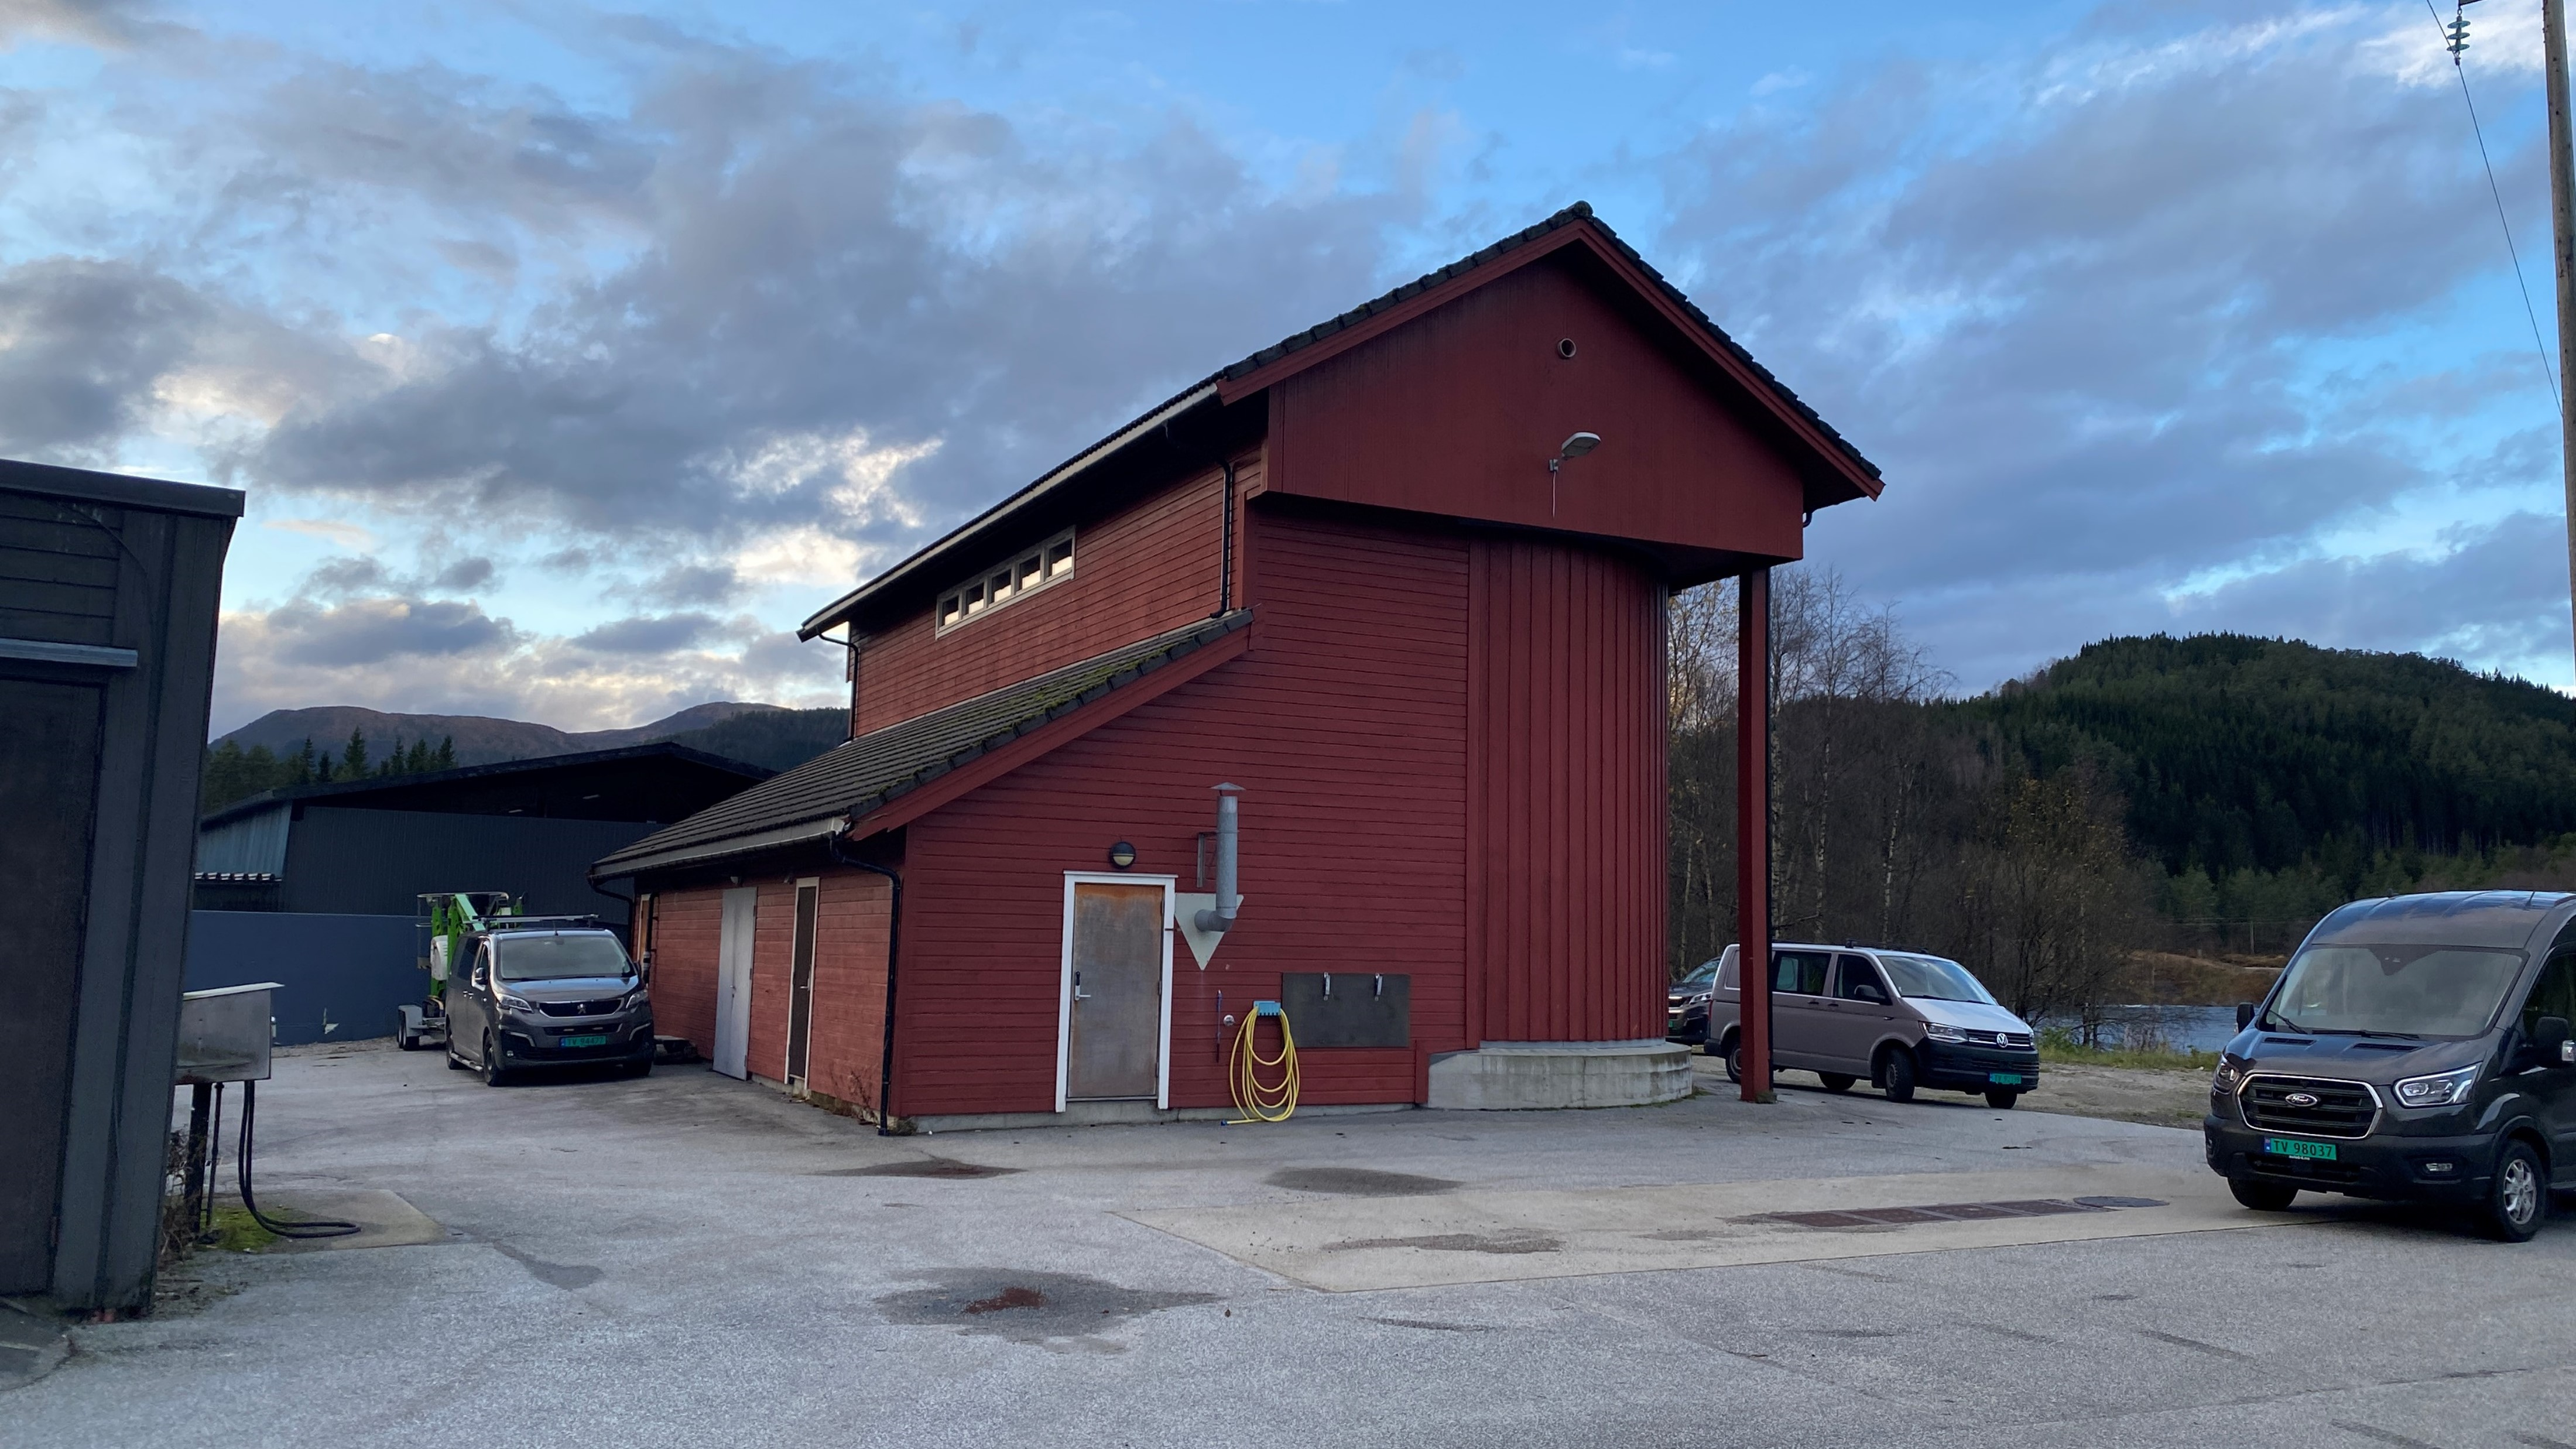
\includegraphics[width=1.1\textwidth]{Bilder/Framside RA200.jpg}
\end{adjustbox}

	\chapter{Forord}
\thispagestyle{romanpages}


Denne rapporten er skreven på vegne av \gls{Renasys}\citep{Renasys} og \gls{Sunnfjord Kommune}\citep{SunnfjordKommune}, i emnet
ELE350-1 23H Bacheloroppgave. Vi starta prosjektet i Januar og er ferdig i slutten av mai.

-- Lage noko eige for takk?

Tusen takk til arbeidsgivarar Renasys og Sunnfjord kommune som har gjort denne oppgåve mogleg.
Tusen takk til alle som har hjelpt og bidratt til arbeidet med denne bacheloroppgåva og
takk til MidTechnolegies og HVL for aktuelle lisensar brukt i oppgåva.

Spesiell takk til familie og vennar som har støtta oss i denne prosessen.


% Bør innehalde
% - Hvorfor arbeidet ble utført
% - Personlige motivasjoner eller inspirasjoner for prosjektet
% - Hvordan prosjektet utviklet seg, eventuelle utfordringer underveis
% - eventuelle spesielle forhold eller omstendigheter rundt forskningen

-- Flytte introduksjon av oss hit ? \newline
-- Flyttes til appendix? All kode for denne bacheloroppgåva er samla i ein felles github (SETT INN LINK)

	\chapter{Samandrag}
\thispagestyle{romanpages}

Bacheloroppgåva, som vi har løyst i saman med \gls{Renasys} og \gls{Sunnfjord Kommune}, handlar om utbetring av styresystemet på 
avlaupsreinseanlegget i Sande i Sunnfjord. 
Anlegget er teknisk utdatert noko som gjer at oppgradering av styresystemet undersøkjast.

Rapporten legg til rette for fire ulike løysningsalternativ
der ulik grad av dybde blir presentert og vurdert. \newline
Rapporten legg til grunn val av løysningsalternativ C der alternativet bygger på planlegginga av eit nytt styresystem.
Rapporten undersøkjar og forklarer generell verkemåte til eit avlaupsreinseanlegg og 
vidare forklarer og dokumenterar reinseanlegget på Sande.

Oppgåva gir innblikk i dei relevante stega i planlegging av eit nytt styresystem der eigen dokumentasjon er brukt som grunnlag for vidare arbeid. 
Utføring av programmering, simulering og testing er løyst med eigne funskjonsblokker og metodar i programmeringsverktøyet \gls{Codesys},
der annerkjende \gls{IEC} standarar er undersøkt og tatt i bruk.
Vidare blir styresystemet og programmeringsarbeidet skildra og dokumentert.

Resultatet av bacheloroppgåva gir vår arbeidsgivar ny og forbetra dokumentasjon av anlegget 
og grunnlaget for eit nytt, fleksibelt og teknisk moderne program. 
Rapporten undersøkjer også generelle oppgraderingar og ytterligare forbetringspotensial 
for reinseanlegget og programmet.

	%--------------------Innhaldsliste / Figurliste / tabell liste---------------------	
	% innholdsliste
	\cleardoublepage
	\pagestyle{romanpages}
	\tableofcontents
	\thispagestyle{romanpages}  % Apply to the first page of the Table of Contents

	\cleardoublepage
	\pagestyle{romanpages}
	\listoffigures
	\thispagestyle{romanpages}  % Apply to the first page of the List of Figures
	
	\cleardoublepage
	\pagestyle{romanpages}
	\listoftables
	\thispagestyle{romanpages}  % Apply to the first page of the List of Tables

	% Turn on the style
	\pagestyle{fancy}


	\clearpage
	\pagenumbering{arabic}
	%\setcounter{page}{5}

	%------------------------------------------------------

	%------------------ Lim inn sider til documentet her ------------------------



	% Kapittel 1 Innleiing
	
\thispagestyle{fancy}

\section{Om oss}

Vi er tre studentar som studerar Automasjon med robotikk ved HVL campus Førde.
Vi har alle fagbrev som elektrikar og fant lett tonen i starten på studiet.
Igjennom tre år har vi brukt vår breie kompetanse innen industri, programmering og elektronikk
til å danne eit godt team.

Fyll inn?



	\section{Oppdragsgivar}
\textbf{Renasys AS i samarbeid med Sunnfjord kommune}

Renasys er ein startup som arbeider med banebrytande teknologi innan mekanisk finpartillekfiltering av avlaupsvatn.
Renasys har 14 tilsette fordelt på kontor på Øyrane i Førde og Sandnes i Rogaland. 
Renasys har lenge arbeida konfedensielt men har gått offentleg med teknologien sin iløpet av 2023. 
Renasys tilbyr reinsetjenester til kommunar og interkommunale selskap innan avlaup og maritim sektor.

Renasys og Sunnfjord kommune arbeider ilag mot Mission Zero som innebærer 
null utslepp, null avfall, null energi og ein generell modernisering av avlaupssektoren i Norge.
Sunnnfjord kommune er ansvarleg for vann, veg og avlaup i sitt område og har bedt 
Renasys om å undersøke moglegheiter for forbetringar av reinseanlegget på Sande i Sunnfjord.
\newline
\newline

\begin{figure}[htbp]
    \centering
    \begin{subfigure}[b]{0.3\textwidth}
        \centering
        
\includegraphics[width=1\textwidth]{Bilder/renasys.png}
        \caption{Logo Renasys}\label{fig:subfig1}
    \end{subfigure}
    \hfill
    \begin{subfigure}[b]{0.3\textwidth}
        \centering
        
\includegraphics[width=0.7\textwidth]{Bilder/SK.png}
        \caption{Logo Sunnfjord kommune}\label{fig:subfig2}
    \end{subfigure}
    \caption{Logo oppdragsgivar}\label{fig:Illustrasjon-Diffuser}
\end{figure}

	% Kapittel 2 Analyse av problemet
	\chapter{Analyse av problemet}
\thispagestyle{fancy}
Her kan vi starte underlaget for kappittelet
	\section{Problemstilling}
Reinseanlegget er teknisk utdatert og er avhengig av modernisering. Stryringssystemet er over tjue år gammalt
og består hovudsakeleg av eldre og utgåtte komponentar. Med gamle komponentar aukar risikoen for svikt, 
og reservedelar som passar kan være vanskeleg å finne.

WaterCare, som leverte styresystemet er i seinare tid også blitt avvikla noko som gjer at kompetansen 
og moglegheiten for å gjere endringar i styresystemet er vankeleg. 
Mykje grunna denne utfordrina har ikkje anlegget følgt den teknologiske framdrifta 
og små problem har samla seg opp til å bli større utfordringar.

Samtidig med desse faktorane er dokumentasjonen til reiseanlegget dårleg noko som gjer at enkle arbeidsoppgåver blir lange og tunge.
I eit værste tilfelle vil styringseinheten på anlegget svikte og med det som er nevnt tidlegare vil det være krevjande
å få anlegget i drift igjen. Dette er eit kritisk problem innan avlaupshandtering og kan ikkje sjåast vekk ifrå.
\newline

\begin{figure}[htbp]
    \centering
    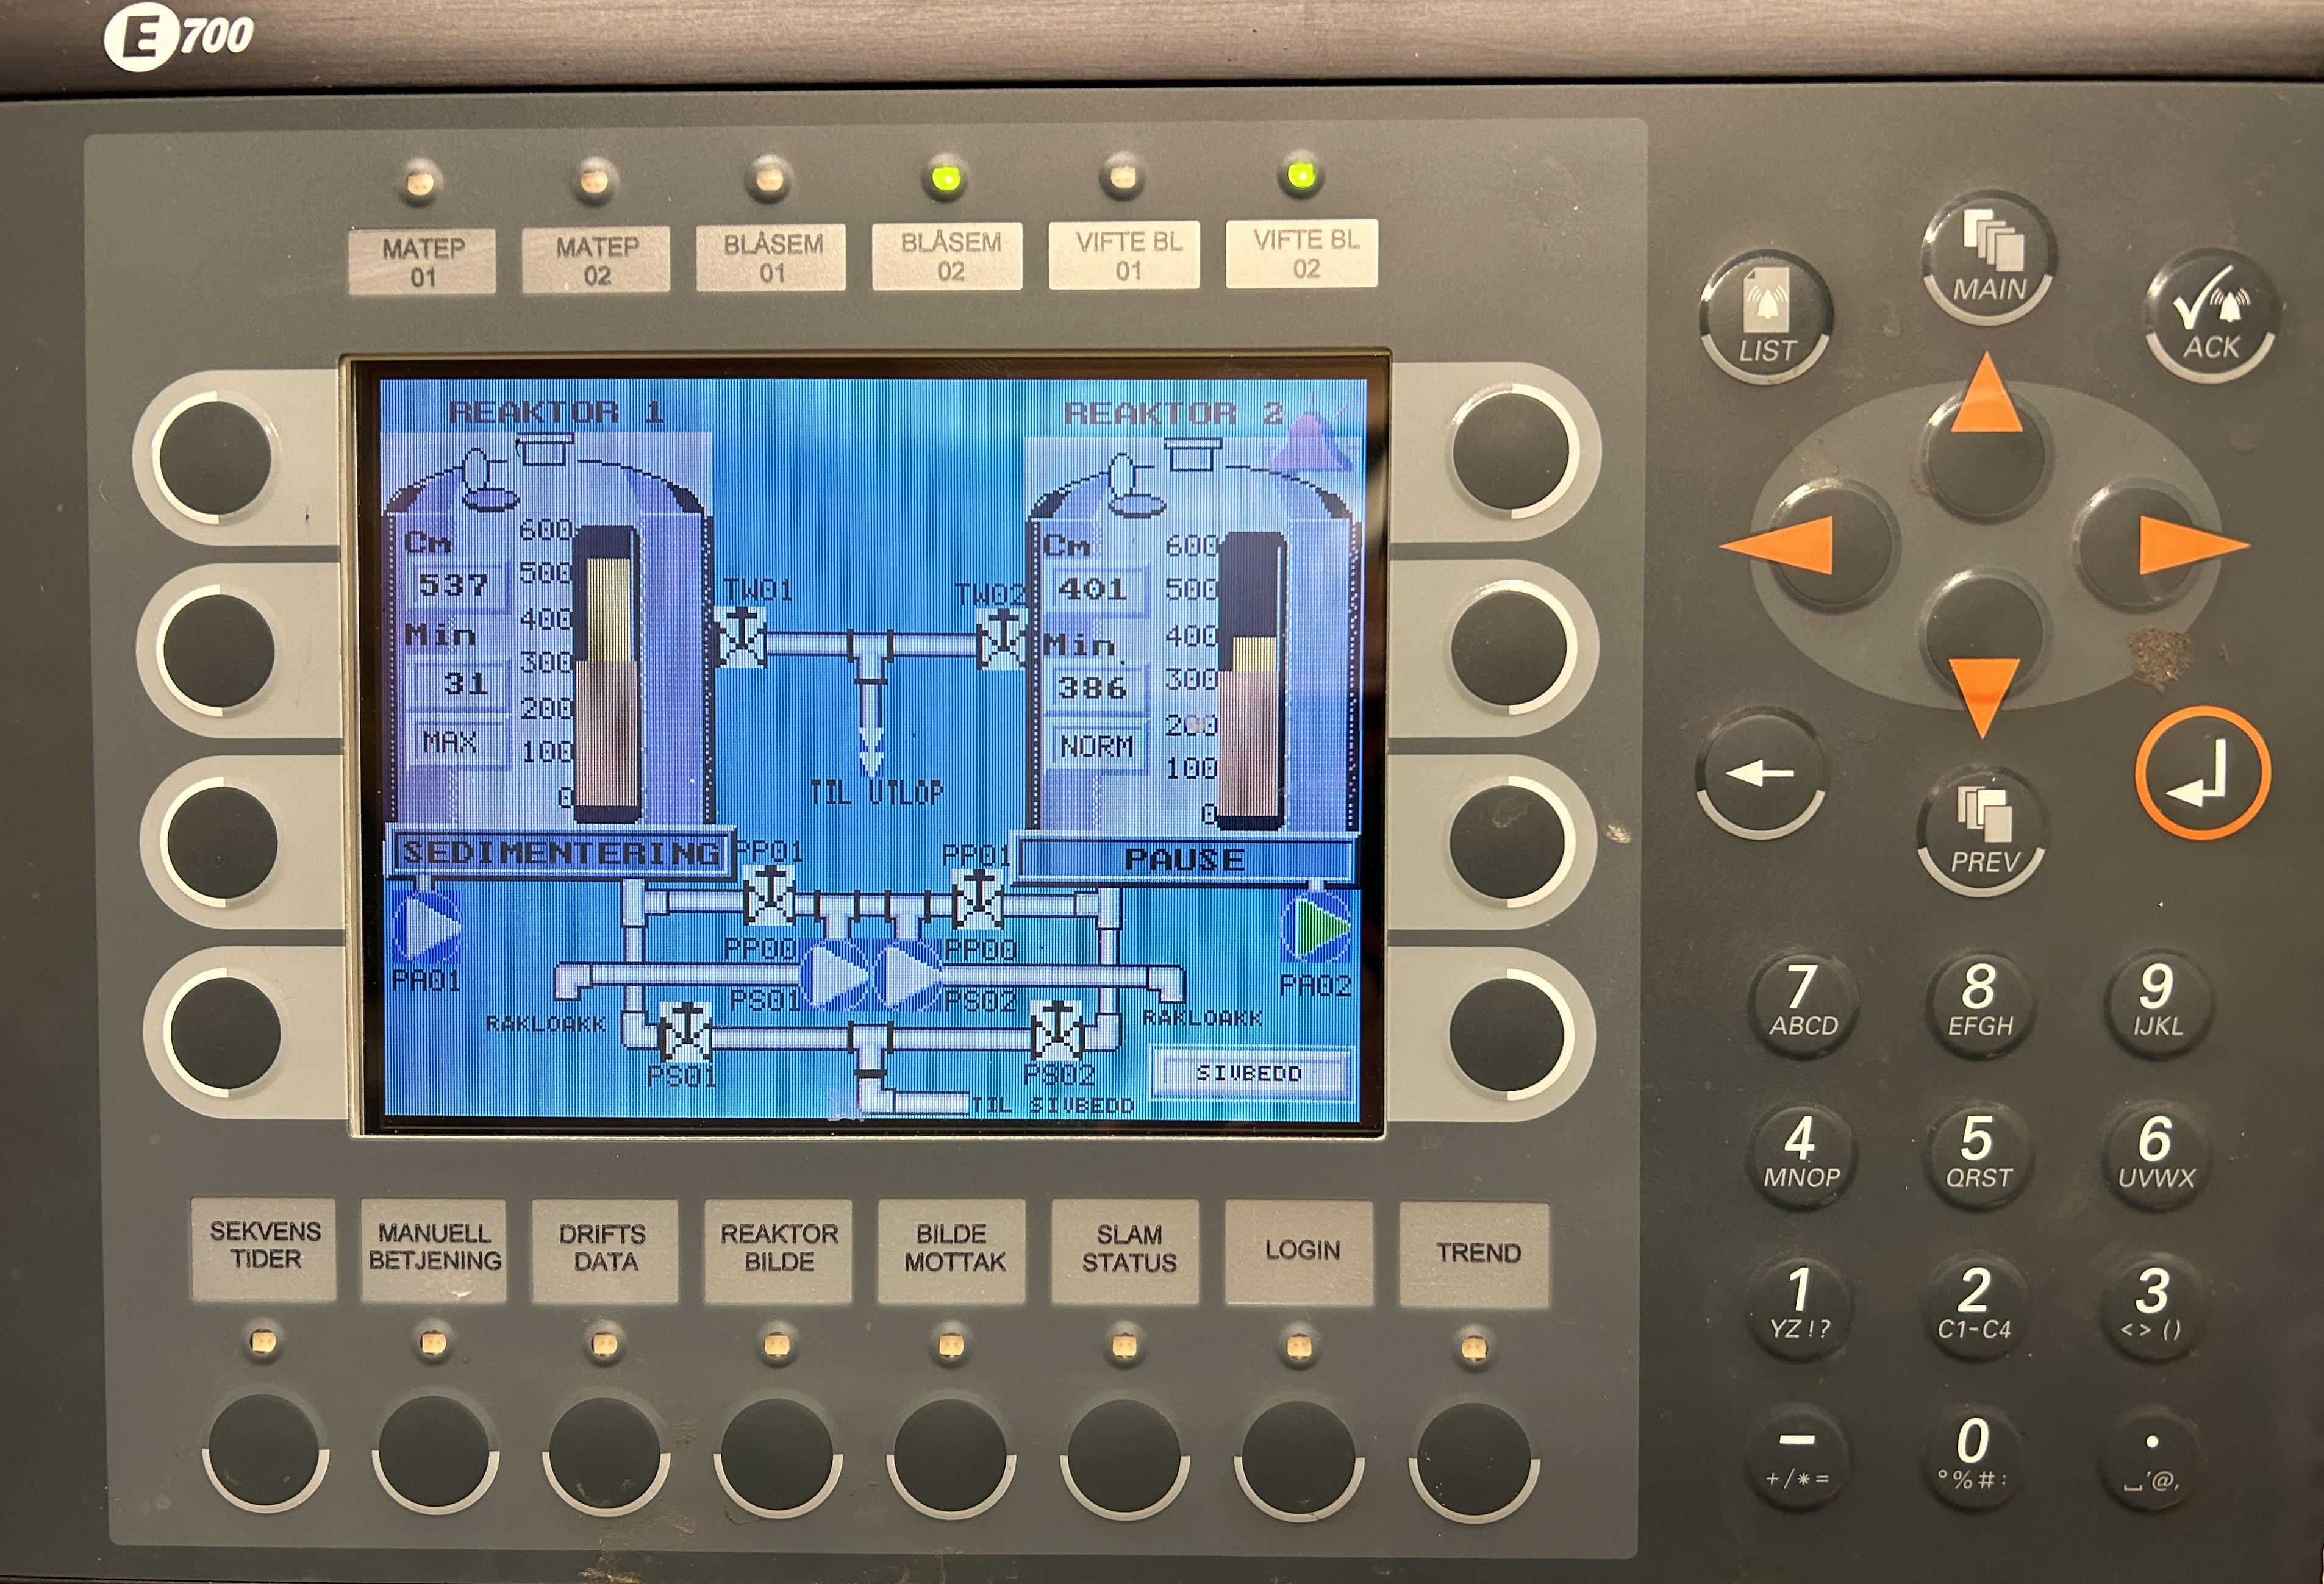
\includegraphics[width=0.8\textwidth]{Bilder/BeijerSkjerm.JPG}
    \caption{Beijer HMI}\label{fig:HMI}
\end{figure}
	\input{Tekst/Kapittel2 - Analyse av problemet/2.2 - Løysningsforslag.tex}
	\input{Tekst/Kapittel2 - Analyse av problemet/2.3 - Val og drøfting.tex}
	
	% Kapittel 3 Krav og mål
	\chapter{Krav og mål}
\thispagestyle{fancy}
Krav i frå \gls{Renasys} var at vi skulle bli einige med \gls{Sunnfjord Kommune} om ein kravspesifikasjon.
Vi hadde eit møte med \gls{Sunnfjord Kommune} der dei hadde nokon konkrete ønsker til oppgåva.

\begin{enumerate}
    \item Vekk frå høge lisenskostandar og skifte ut pls
    \item Betre og ny dokumentasjon, med bl.a.\ funksjonsbeskrivelse
    \item Klargjering av styresystemet for nye komponentar som ein forbertring av anlegget
\end{enumerate}

\section{Krav}
Vi brukte dei overnemnde krava til \gls{Sunnfjord Kommune} til å forme kravspesifikasjon vår.
Derretter utarbeida vi ei liste med krav der det vart naturleg og dele dette opp i tre
hovuddelar; dokumentasjon, programering og simulering med verifisering. Dette gjorde vi i samråd med rettleiar
og fekk dette godkjent av oppdragsgivarane våre.

\begin{enumerate}
    \item Dokumentasjon med detaljert funksjonsbeskrivelse som innheld bl.a.
        \begin{itemize} 
        \item Anleggets verkemåte
        \item Blokkdiagram
        \item Interlock-liste
        \item IO-liste
        \item objektliste
        \item Alarmliste
        \item Eletriske teikningar
        \item P\&ID
        \item Vedlikehaldsmanual
        \end{itemize}
    \item Programmering
        \begin{itemize}
        \item Bruke ny funksjonsbeskrivelse som base
        \item Bruke open kjeldekode og ikkje låse seg til leverandør
        \item etter IEC 61131\textemdash3 standard
        \end{itemize}
    \item Simulering med verifisering
        \begin{itemize}
        \item Lage eit sumleringsverktøy for å teste koden
        \end{itemize}
\end{enumerate}

bruke Open source codesys programmering
- ikkje dyrt, enkelt og vedlikehalde
- Ikkje låse seg til ein leverandør

\section{Mål}
Det er nokon mål me har lyst og oppnå for dette systemet.

\begin{itemize}
    \item Programmere fire IEC blokker: MB,MA,SBE og SBE
    \item program som er enkelt og vedlikehalde
\end{itemize}

\section{Oppgraderingar}

Dette var ekstra ønsker frå kommunen i forhold til programmet. 

	% Kapittel4 - Anleggets Verkemåte
	\chapter{Anleggets verkemåte}
\thispagestyle{fancy}

Første steg i løysninga var å sette seg inn i anleggets verkemåte.\newline
For å setje oss in i korleis Sande reinseanlegg fungerar var vi nødt til å forstå
korleis eit generelt avlaupsreinseanlegg er bygd opp.



	\section{Generel verkemåte}

Eit avlaupsreinseanlegg er bygd opp av 3 hovuddelar: Primær, sekunder og tertiærreinsing.
Alle desse delane kan løysast på forskjellige måtar, men hovudoppgåvene er dei same
i alle reinseanlegg.

Primærreinsing handlar om å skille organisk og uorganisk materiale.
I eit avlaupsreinseanlegg tilsvarer dette å skille avlaupsvatnet, 
som ein vil behandle frå, sand, Q-tips, våtserviettar
og anna uønska material som ein ikkje ynskjer vidare i prosessen. \newline
Primærreinsing er eit viktig steg for å beveare pumper og anna prosessutstyr.

Sekunderreising handlar om å fjerne mest mulig suspanderte stoffer og organisk materiale.
Det tilsvarer å skilje det meste av organisk materialet frå vatnet.
Sekunderreising er i kvart anlegg avhengig av kva `reinseprinsipp' som er brukt. Dette tilsvarer
kva teknolgisk metode som nyttast for å utføre dette steget.

Tertiærreising handlar om å fjerne resterande forureiningar i vatnet.
Dette steget varierer veldig frå anlegg til anlegg og eg er
avhengig av kva krav reiseanlegget har som krav på sitt utslippsvatn.

\begin{figure}[htbp]
    \centering
    \includegraphics[width=1\textwidth]{Figurar/Generellverkemåte.png}
    \caption{Generell verkemåte for eit avlaupsreinseanlegg}\label{fig:HMI}
\end{figure}

Når vi hadde satt oss inn i den generelle verkemåten til eit avlaupsreinseanlegg
valgte vi å fokusere mot Sande.
Dette valgte vi å gjere i tre hovuddelar. Kva teknologisk reinseprinsipp er brukt, korleis er Sande reiseanlegg
kopla opp mot teknologien teoretisk og korleis fungere reinseanlegget praktisk tjue år etter innstalasjon.
	\newpage
\section{Teknologisk Verkemåte}
\thispagestyle{fancy}
Sandre reinseanlegg er konstruert basert på SBR-teknologi

SBR står for `Sequence Batch Reactor', på norsk `sekvensiell batchreaktor'.\newline
SBR er en reinsemetode basert på aktiv slam der alle prosessar føregår i same reaktortank. 
Reaktor nyttar biologisk reinsing med mikroorganismar for å koagulere 
og fjerne løyste og ikkje sedimenterbare partiklar samt stabilisere organisk materiale. 
Avløpsvatn tilførast reaktor i «batcher» for å bli reinsa og uttappa. 
Kvar avløps-batch går igjennom ein reaktorsekvens som består av følgande fem delsekvensar.
\newline

\begin{figure}[htbp]
    \centering
    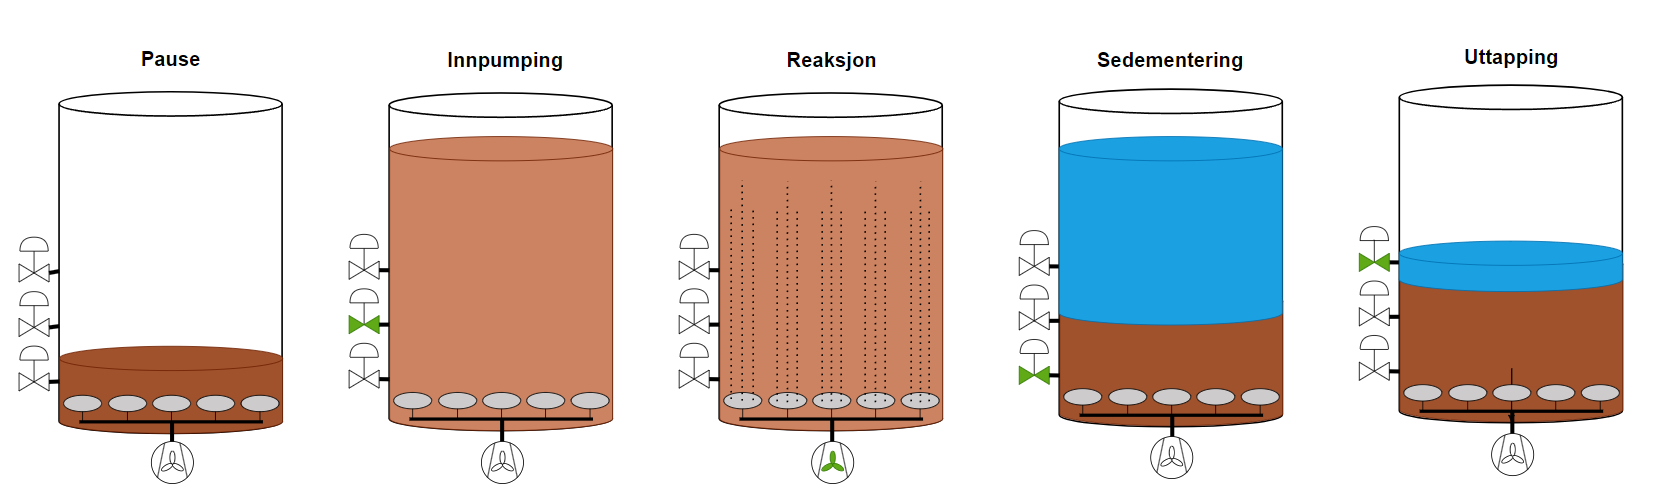
\includegraphics[width=1\textwidth]{Figurar/SBR-V2.png}
    \caption{SBR-prossessen}\label{fig:HMI}
\end{figure}


\begin{enumerate}
    \item \textbf{\makebox[3cm][l]{Pause}:} Reaktoren venter til det er behov for dens kapasitet.
    \item \textbf{\makebox[3cm][l]{Innpumping}:} Reaktoren mottar avlaupsvatn, normalt ifrå ein utjamningstank.
    \item \textbf{\makebox[3cm][l]{Reaksjon}:} Reaktoren periodisk luftast for å tilføre oksygen til mikroorganismane.
    \item \textbf{\makebox[3cm][l]{Sedementering}:} Reaktoren sedementerer ved hjelp av gravitasjon. Overskudd slam fjernast.
    \item \textbf{\makebox[3cm][l]{Uttapping}:} Reaktoren drenerar reisa vatn mot resepient.
\end{enumerate}

Meir detaljert informasjon om SBR og anleggets teknolgiske prinsipp er tilgjengeleg i anleggets
funksjonsbeskrivelse. (INSERT APPENDIX REFERANSE MED LINK)


	\newpage
\section{Teoretisk Virkemåte}
\thispagestyle{fancy}


% Sande reinseanlegg består av primærreinsing via ein grovrist. Frå grovrista
% rennet vatnet med sjølvfall til ein mottakstank som fungerar som utjamningstank og samlar varierande tilstrøymingar 
% for å gi resten av anlegget homogene forhold. 
% Vidare blir vatnet pumpa frå mottakstanken opp til ein av reaktorane.
% Innpumping skjer til den reaktoren som er i riktig fase og er klar for ny batch.
% Sekundær og tærtierreinsing skjer i desse reaktorane som anvender SBR-teknologi.

% Dersom ingen av reaktorane er i riktig fase vil avlaupsvatnet lagrast i mottakstanken
% heilt til ein av reaktorane har avslutta sin syklus.
% Avlaupsvatnet vil opphalde seg i eller på veg mot ein av desse fire hovuddelane medan det er i anlegget.

Sande reinseanlegg består av primærreinsing via grovrist, ein mottakstank 
som samlar varierande tilstrøymingar for å gi resten av anlegget homogene forhold og
sekundær og tærtierreinsing ved to reaktorar som anvender SBR-teknologi.

Avlaupsvatnet vil opphalde seg i eller på veg mot ein av desse fire hovuddelane medan det er i anlegget.
Ferdig behandle avlaupsvatn blir drenert ut til resepienten Gaula. 
Gaula er ei elv som renn ifrå Hestad, forbi Sande og munner ut i Dalsfjorden.

\begin{figure}[htbp]
    \centering
    \includegraphics[width=1\textwidth]{Figurar/Sande verkemåte.png}
    \caption{RA200 flytskjema}\label{fig:HMI}
\end{figure}

\subsection{Grovrist}
Innløpet på anlegget renn først igjennom grovrista. Grovrista på reinseanlegget
er ein (Huber rotomat R09). Grovrista fungerer som ein liten tank og ein nivågivar starters
skruen ved innkommande avlaupsvatn. Skruen tek med unøska materiale og fjernar det til eigen avfallshandtering.
Dersom grovrist feile vil vatnet renne vidare via overløpsrøyr.

\newpage
\subsection{Mottakstank}
Frå grovrista renner vatnet med sjølvfall mot mottakstanken som ligger som lavaste punkt på anlegget.
Mottakstanken er 120 $m^3$ og er ein felles lagringsplass for vatnet før det går vidare mot reaktorane.
Mottakstanken har fire sensorar som heng ifrå taket.

\begin{itemize}
    \item Trykkgivar for nivå (PP00-LT01)
    \item Trykkgivar for overløp (PP00-LT02)
    \item Flottør-vippe lav (PP00-LS02)
    \item Flottør-vippe høg (PP00-LS01)  
\end{itemize}

Nivået i mottakstanken blir primært målt med trykkgivar LT01. For at vatnet skal pumpast vidare mot ein
reaktor i riktig sekvens må trykkgivar indikere at nivået er høgt nok. LS02 fungerar som backup.
I toppen av mottakstanken er det ei overløpskasse som drenerer mot resepient, her vil det
ved normale omstendigheter ikkje renne anna ein reinsavatn. Trykkgivar for overløp måler
dersom ureinsavatn renner i resepientrøyret.

%% Må endre på tegning fordi det eine navnet er feil. Ikkje reject frå sivbed.

\begin{figure}[htbp]
    \centering
    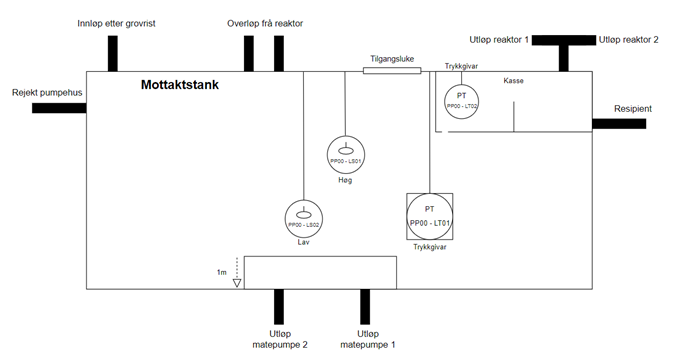
\includegraphics[width=1\textwidth]{Figurar/Mottakstank.png}
    \caption{Illustrasjon mottakstank}\label{fig:HMI}
\end{figure}

\newpage
\subsection{Reaktor}


	\newpage
\section{Praktisk Virkemåte}
\thispagestyle{fancy}

Sjølv om Sande reiseanlegg anvender SBR-teknologi så er det enkle spesefikke
punkter der dette reiseanlegget avviker ifrå normen. 
Sande reinseanlegg bruker eksempelvis ein spesiel form for slambehandling sett i norsk perspektiv.

Vanleg slambehandling i Noreg er oppsamling av slammet i tanker som handterast og tømmast av lokale etater.
På Sande blir ikkje slammet lagra, men jamnlig spreid ut over eit designert område. På dette området er
det planta siv som skal ta opp slammet og det resterande vatnet blir naturleg filtrert og drenert.
Desse områda kallast sivbed.

Sivbeda er konstruert med fleire dreneringslag som gjer at resterande vatn skiljast ut i designerte soner.
Her kan desse handterast vidare etter ønska behov. 
Grunna denne slambehandlingsmetoden er det på Sande reiseanlegg heller slamfjerning frå reaktor
i reaksjonsfasen. Dette blir gjort for å ha mindre konsentrert slam.

Sande reiseanlegg har fire sivbed med kombinert størrelse på 676 kvadratmeter, som står på utsida av reiseanlegget.


\begin{figure}[htbp]
    \centering
    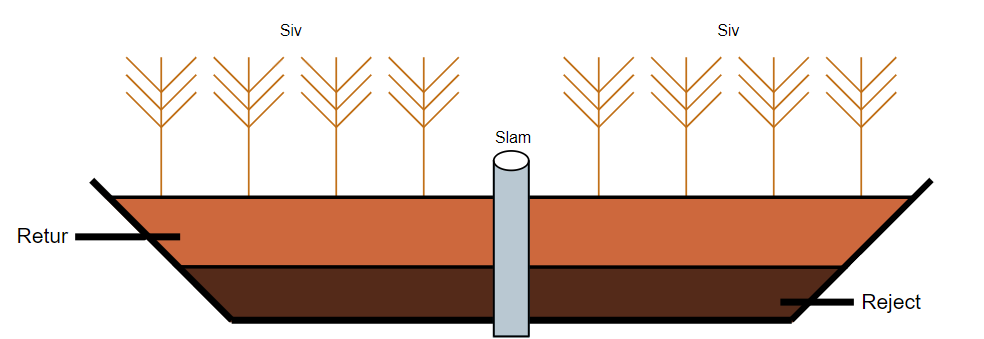
\includegraphics[width=1\textwidth]{Figurar/Sivbed.png}
    \caption{Illustrasjon sivbed}\label{fig:HMI}
\end{figure}


\newpage

Vatnet frå desse forskjellige dreneringslaga blir samla til eit pumpehus/komme.
Dette pumpehuset står ca femti meter ifrå sjølve reinseanlegget og er utstyrt med to pumper og nokre nivåbrytarar.
Pumpekommen er delt i to og skiller på vatnet som kjem ifrå dei forskjellige dreneringslaga. \newline
På Sande reiseanlegg er djupaste dreneringssona klassifisert som rein reject og blir sendt ut til resepient.
Den øvre dreneringssona er forsatt klassifisert som skitten og blir returnert til mottakstanken.

\begin{figure}[htbp]
    \centering
    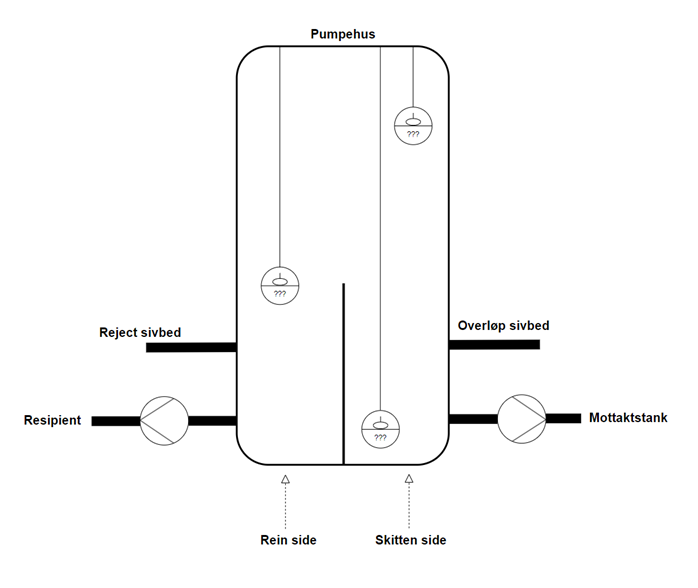
\includegraphics[width=1\textwidth]{Figurar/Pumpehus.png}
    \caption{Illustrasjon pumpehus}\label{fig:HMI}
\end{figure}

\newpage




	\newpage
\section{Dokumentasjon}
\thispagestyle{fancy}

Som tidlegare spesifisert i kapittel 3 var ein stor del av oppgåva vår og dokumentere
anlegget og verkemåten til anlegget. Vi bestemte oss for å gjere ei dokumentasjonsfornying,
altså at vi henta det som var av tidlegare dokumentasjon og kombinerte det med vår nyerfarte kunnskap.

Vi oppretta ein funksjonsbeskrivelse som bygger vidare på driftsinstruksen som var levert av 
Watercare i 2003. Dokumentet er tiltenkt ein slags bruksanvisning på heile anlegget,
der sikkerheit, prosess, verkemåte og programmering er sentrale tema. \newline
Funksjonsbeskrivelsen skal være forståeleg for alle parter som har interesse i reinseanlegget
og både driftspersonell og programmerere skal kunne få eit godt innblikk i anlegget.

Funksjonsbeskrivelsen inneheld alt om reinseanlegget på Sande men er delt opp i kapittel for å ikkje
overvelde lesar med mykje unødvendig informasjon. Desto lenger ned i dokumentet ein kjem jo meir avansert blir infomrasjonen
og programmering av anlegget ligger under udjupa teknisk beskrivelse.

Dokumentet er delt opp i desse kapittela

\begin{enumerate}
    \item Introduksjon
    \item Verkemåte
    \item Teknisk beskrivelse
    \item Drift og vedlikehald
    \item Feilsøking
    \item Utdjupa teknisk beskrivelse
    \item Teknisk underlag
\end{enumerate}

Alt som er nemnt her i kapittel 4 står meir detaljert under kapittel Teknisk beskrivelse i funksjonsbeksrivelsen, og
er sentralt for å best forstå korleis anlegget fungerer.

Funksjonsbeskrivelsen i sin heilhet ligger som vedlegg (SETT INN VEDLEGG)

	% Kapittel 5 - Tilrettelegging for programmering
	\chapter{Tillrettelegging for programmering}
\thispagestyle{fancy}

Som tidlegare beskrive under krav og mål, ønska vi å bruke ein løysning som ikkje har løypande lisenskostnadar for vår sluttkunde. 
Sunnfjord kommune var veldig interessert i å ikkje låse seg til ein fast leverandør, men heller ha moglegheita til å ha valet mellom fleire 
leverandørar innan levering av PLS. Dette gjorde at vi såg vekk ifrå Siemens TIA-portal som vi hadde lært
igjennom PLS faget, og begynte å sjå i andre endar.
Programmet ønska vi å skrive i Structured Text (ST) men fikk også anbefalt typar av grafiske diagram baserte språk for å lettare
vise sammenheng i programmet.

Det var også viktig at alle på gruppa kunne programmere samtidig og at ein felles programmeringsstandard skulle nyttast.
Det var viktig at parralelt arbeid ikkje skulle by på synkroniseringsproblemer og at det var ei god løsyning for dette.

	\section{Codesys}
\thispagestyle{fancy}
Som tidlegare beskrive under krav og mål, ønska vi å bruke ein løysning som ikkje har løypande lisenskostnadar for våra sluttkunde. 
Kommunen var veldig interessert i å ikkje låse seg til ein fast leverandør, men heller ha moglegheita til å ha valet mellom fleire leverandørar innan levering av PLS, så valet falt på programeringsplattforma Codesys\citep{Codesys} laga av Codesys Group. 
Codesys tilbyr ein open kildekode løysning for prosjekta, og har ingen lisenskostnadar for sluttkunden. 
I tillegg så kan prosjektfilane brukast på fleire typar PLS einingar. 
Dette gir våra sluttkunde fleksibilitet i korleis dei ønska å implementere våra løysningsforslag til deira anlegg.

Codesys nyttar programeringsspråkstandaren satt av IEC 61131 som blant anna Structured Text (ST), Sequential Function Chart (SFC) og Ladder Diagram (LD). I våra program er all logikk skrevet i strukturert tekst (ST), og bygd opp av ein blokk-basert programering med Continuous Function Chart (CFC). 
CFC er en grafisk programmeringsspråk som utvidar dei standardiserte språkene i standarden og gir koden ein god lesbarhet.

Codesys har nyleg fått støtte for integrering av Github i programmvaren, som gjer det mykje enklare for oss å halde versjonskontroll og enkelt for fleire av gruppemedlemmene å kode saman på same prosjekt. 
Denne funksjonaliteten har vi nytta oss av flittig, og har hjelpt oss med å kunne ha moglegheita til å jobbe individuelt med prosjektet.

Vidare så har Codesys støtte for bibliotekar igjennom CODESYS Store. 
Med å bruke kjente bibliotek så får vi tilgang ei samling av gjenbrukbar kodeblokker, funksjoner og komponentar som vi kan nytte.
Dei biblioteka vi har brukt er som følger:

\begin{itemize}
    \item CODESYS Building Automation \citep{BuildingAutomation}
    \item SysTime \citep{DateAndTime}
    \item Util \citep{DateAndTime}
\end{itemize}

\newpage
	\section{IEC}
\thispagestyle{fancy}

\gls{IEC} \citep{IEC} er ein internasjonal, ikkje statleg orginasjon som utviklar og publiserer tekniske standardar innan elektrofag. 
Norge er representert i IEC ved Norsk Elektrotekniske Komité (NEK) \citep{IEC-SNL}. 
IEC har standarar som dekker programmering av PLS som går heilt tilbake til 1993\citep{Wiki-93}. 
Den nåverande standaren som omfavner PLS er IEC 61131\citep{IEC-61131}. Dette er ein standar spesielt designet for programmerbare kontrollera, og er delt opp i 10 delar, der del 3 tar for seg programmeringsspråk. 

Våra program er programmert i hovudsak etter IEC 61131-3 og IEC \gls{PAS} 63131\citep{IEC-63131}. 
Der IEC PAS 63131 er ein standard utarbeida av IEC som gir oss grunnlag for å lage \gls{SCD} samt å bruke forhandsdefinerte funksjonstemplater for funksjonsblokker. 
IEC PAS 63131 er laga med formål at leverandørindustrien og oljeselskap skal ha et felles rammeverk for bruk på norsk sokkel, og er utarbeida etter NORSOK I-005:2013.
Med å bruke desse standardane så gir det oss eit robust og fleksibelt rammeverk for å programmerer anlegget. 
Ved bruk av dei forhandsdefinerte funksjonsblokkane har vi moglegheit til å enkelt knytte i hop fleire delar av programmet våra, og ha fleksibilitet ved å enkelt kunne endre og legge til funksjonar i programmet. 
Dette er noko vi har heile vegen har fokusert på, da våra sluttkunde har heile vegen ytra eit ønske om å ein del tilleggsfunksjonar i programmet, utover det som er der i dag. 

Vi bestemte oss for å lage 4 funksjonsblokker (MB, MA, SPV, SPE) i frå IEC 63131 for å få dekka behovet for dei objekta (sensor, ventil og motorar) vi hadde for å kunne programmere anlegget i sin heilheit. 
Blokkene blei laga med full funksjonalitet etter standaren, enda vi ikkje vi ikkje hadde behov for  alle funksjonane som var i standaren. Med objekt orientert programmering kan ein enkelt skalere frå 1 til 10 sensorar, med veldig lite koding, slik at desse kan lett dupliserast ved seinare anledning om det er ønskjeleg med utviding av koden med nye funksjonalitetar. 


	
	\section{SCD}
\thispagestyle{fancy}

Etter vi hadde valgt dei blokkene vi ønskte var det naturleg å sette seg ned å planlegge korleis vi ønska å knytte desse blokkene opp i mot anlegget. 
Vi valte da å starte med å lage eit System Control Diagram (SCD) over anlegget. 
Eit SCD er ein grafisk representasjon av anlegget, som visar komponentane i anlegget og deira funksjon, forbindelsar og struktur. 
IEC PAS 63131 standaren gir oss retningslinjene for utforming av diagrammet.


\begin{figure}[htbp]
    \centering
    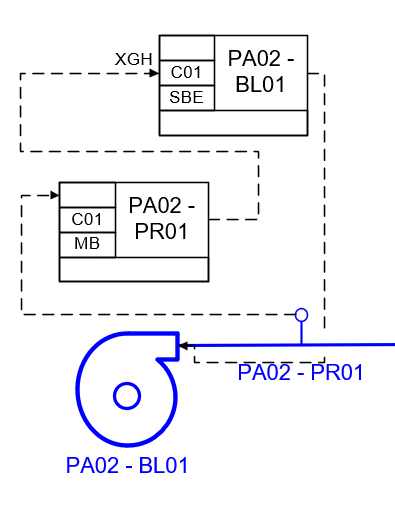
\includegraphics[width=0.35\textwidth]{Bilder/Visio_eksempel.png}
    \caption{Utsnitt frå SCD}\label{fig:SCD eksempel}    
\end{figure}


Første utkast av våra SCD innhald koplingane frå komponentar til blokker og korleis forbindelsane imellom desse skulle fungere. 
Korleis dei forskjellige sekvensane skulle interagere med våra blokker og komponentar var litt uklart for oss på detta stadiet, så vi valte å gå vidare for å starte å lage noko av programmet, slik at vi lettare kunne lage oss eit bilete av korleis vi ville løyse oppgåva.

\newpage
	\section{Tilstandsmaskin}
\thispagestyle{fancy}


Vi identifiserte tidleg i prosessen at vi hadde eit ønskje om å lage ein tilstandsmaskin som hadde den overordna styringa over kvar reaktor. 
Sidan ein SBR tank er prinsipielt oppbygd av forskjellige sekvensar, virka det logisk å lage til ein tilstandsmaskin som gjekk igjennom dei forskjellige tilstandane basert på logikk som vart plassert i dei forskjellige tilstandane. 
Det vart tidleg i prosjektet utarbeida mykje dokumentasjon om verkemåte til anlegget som gjorde at vi kunne enkelt programmere ein tilstandsmaskin som vart intregert mot dei forskjellige sekvensane i anlegget. 
Tilstandsmaskina tar inn signal i frå dei forskjellige tilstandane i anlegget og avansera til neste sekvens når logikken i tilstanden gir signal om at den er ferdig. 

\begin{figure}[htbp]
    \centering
    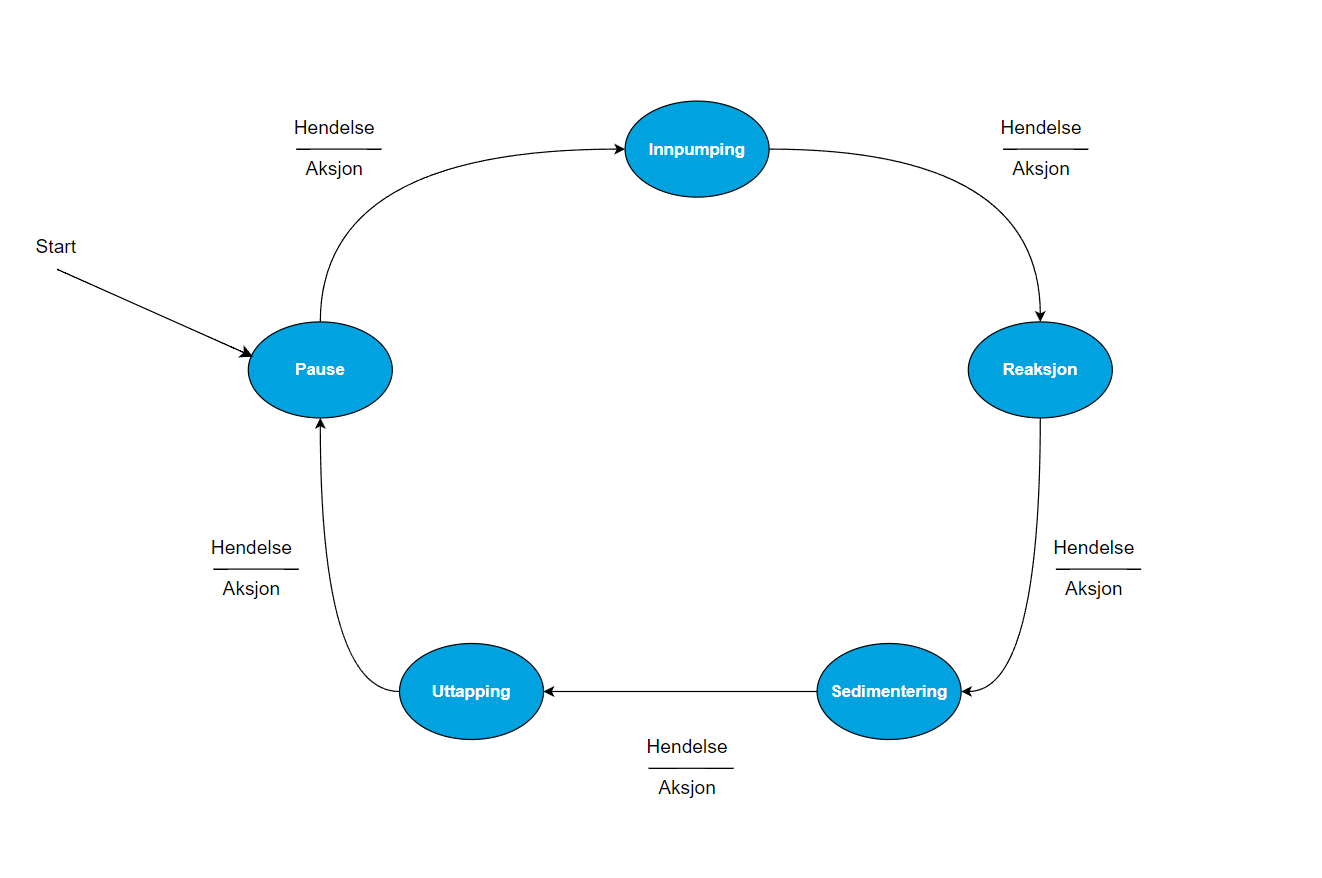
\includegraphics[width=1\textwidth]{Figurar/Tom tilstandsmaskin.png}
    \caption{Tilstandsmaskin prinsipp}\label{fig:Tilstandsmaskin prinsipp}    
\end{figure}

\newpage



	% Kapittel 6 - Programmering
	\chapter{Programmering}
\thispagestyle{fancy}
I dette kapittelet tek vi før oss programmeringa frå start til slutt.

Etter å ha danna oss eit godt grunnlag og eit bilete av korleis vi ønska programmet i kapittel \ref{sec:5} 
begynte vi med programmeringa med eit tomt prosjekt i \gls{Codesys}. Første steget i var å 
settje oss inn i, og programmere \gls{IEC} blokkene som vi valgte i kapittel \ref{sec:5.2}

Undervegs i programmeringa av \gls{IEC} blokkene såg me også nødvendigheita av nokon generelle funksjonsblokker
som kunne gjenbrukast fleire gonger i programmet.


%% CODESYS is a software platform for industrial automation technology. 
%%The core of the platform is the IEC-61131-3 programming tool "CODESYS Development System".


	\section{Programmering av blokker}
\thispagestyle{fancy}

%Skriv OM:
%Programmering av IEC Blokker (MB,MA,SBE,SBV) 
%+ fb blokker (fbTimer, fbAnalougeAlarm, fbCAC)
%- Til appendiks, Heile kode for t.d. fbTimer, fbCAC osv

% Skrive litt om blokka sin funksjonalitet
% Korleis me brukte blokkene i programmet.

\subsection{Monitor Analogue}
\gls{MA} funksjonsblokka er brukt for skalering, visning, overvåking og alarmhandtering av analoge inngangsvariablar i ein prosess.
Funksjonsblokka inneheld supression og blokking funksjonalitet.

Vi bruker \gls{MA} funksjonsblokka er brukt i programmet for å overvåke analoge trykknivågivarar samt å skalere og vise desse som ein fyllingsgrad i prosent.

\begin{figure}[htbp]
    \centering
    \begin{subfigure}[b]{0.45\textwidth}
        \centering
        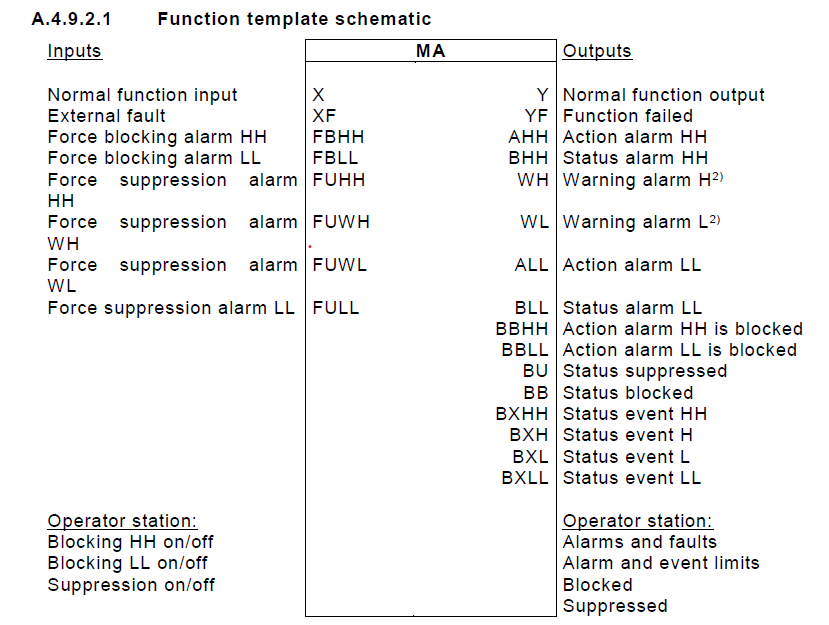
\includegraphics[width=1\textwidth]{Bilder/MABlokkIEC.png}
        \caption{IEC}\label{fig:Monitor Analogue blokk IEC}
    \end{subfigure}
    \hfill
    \begin{subfigure}[b]{0.45\textwidth}
        \centering
        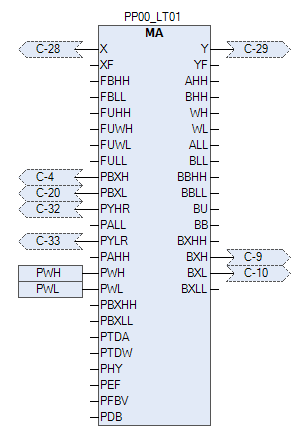
\includegraphics[width=0.7\textwidth]{Bilder/MABlokkIProgrammet.png}
        \caption{Bruk i programmet}\label{fig:Monitor Analogue blokk i programmet}
    \end{subfigure}
    \caption{Monitor Analogue}\label{fig:Monitor Analogue}
\end{figure}
\newpage

\subsection{Monitor Binary}

\gls{MB} funksjonsblokk blir brukt for automatisk overvåking, alarmhandtering, framvising og latching av binære prosess variablar.
Funksjonsblokka inkluderer alarm suppression og blocking funksjonalitet. Funksjonsblokka har moglegheit for invertering av 
inngangssignal og moglegheit for tidsforsinkelse av utgangssignal via parameter.

funksjonsblokka er brukt i programmet for å overvåke alle digitale nivåfølerar i prosessen.

\begin{figure}[htbp]
    \centering
    \begin{subfigure}[b]{0.45\textwidth}
        \centering
        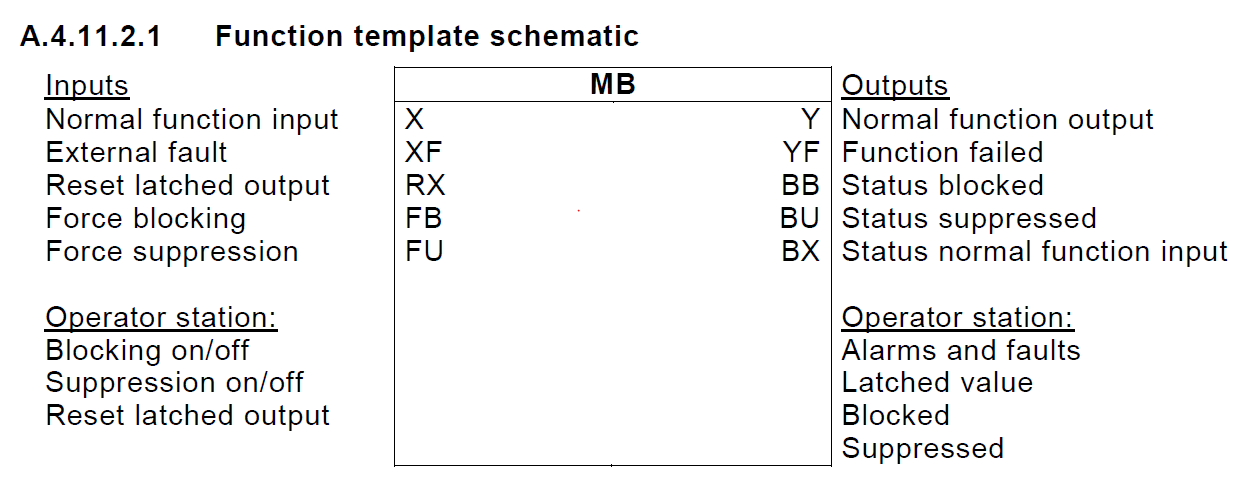
\includegraphics[width=1\textwidth]{Bilder/MBBlokkIEC.png}
        \caption{IEC}\label{fig:Monitor Binary blokk IEC}
    \end{subfigure}
    \hfill
    \begin{subfigure}[b]{0.45\textwidth}
        \centering
        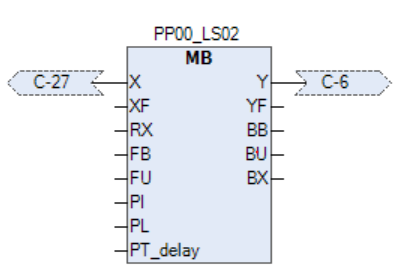
\includegraphics[width=0.7\textwidth]{Bilder/MBBlokkIProgrammet.png}
        \caption{Bruk i programmet}\label{fig:Monitor Binary blokk i programmet}
    \end{subfigure}
    \caption{Monitor Binary}\label{fig:Monitor Binary}
\end{figure}

\newpage

\subsection{Switch Binary Value}

\gls{SBV}-funksjonsblokka skal brukast for binær (på/av) kontroll av eit flyt elelement ved å endra straumen av medium (varme eller væske). 
Typisk kontrollerte element er ventilar, spjeld, osv.

funksjonsblokka er brukt i programmet for styre ein ventilar.

SBV-funksjonsblokka skildrar kontrollen av ventilar med dei binære inngongane XH og XL. Det er ein utgang, Y, som formidlar eit opne/lukke (høg/låg) kommando til ventilaktivatoren, eller dei pulserte utgangane YH og YL kan brukast. Funksjonsblokka har også utgonger XGH og XGL som bekreftar at ventil har fått høg eller låg tilbake melding frå ventilen.
Forklaringa på kontrollfunksjonane (rektangla) er som følgjer: "Kontrollfunksjon": Denne funksjonen utfører fleire oppgåver.
• Den genererer feilstatus YF dersom ein ekstern eller intern feil blir rapportert;
• Den set utgangen Y i samsvar med parameter når feil blir oppdaga;
• Den set utgangen Y basert på tilbakemelding i ytremodus når ingen eksterne inngangar blir brukte (XOH/XOL).
Der er det mogleg og bruke inngongar som kan handtere Lock safeguarding Force safeguarding, force disable transition, Force blocking, Force suppression. Videre er det også inngangar for lock Auto, manuell og outside.
Samt utgonger for som bekreftar status blocked, suppressed, auto/man og outside.

\begin{figure}[htbp]
    \centering
    \begin{subfigure}[b]{0.45\textwidth}
        \centering
        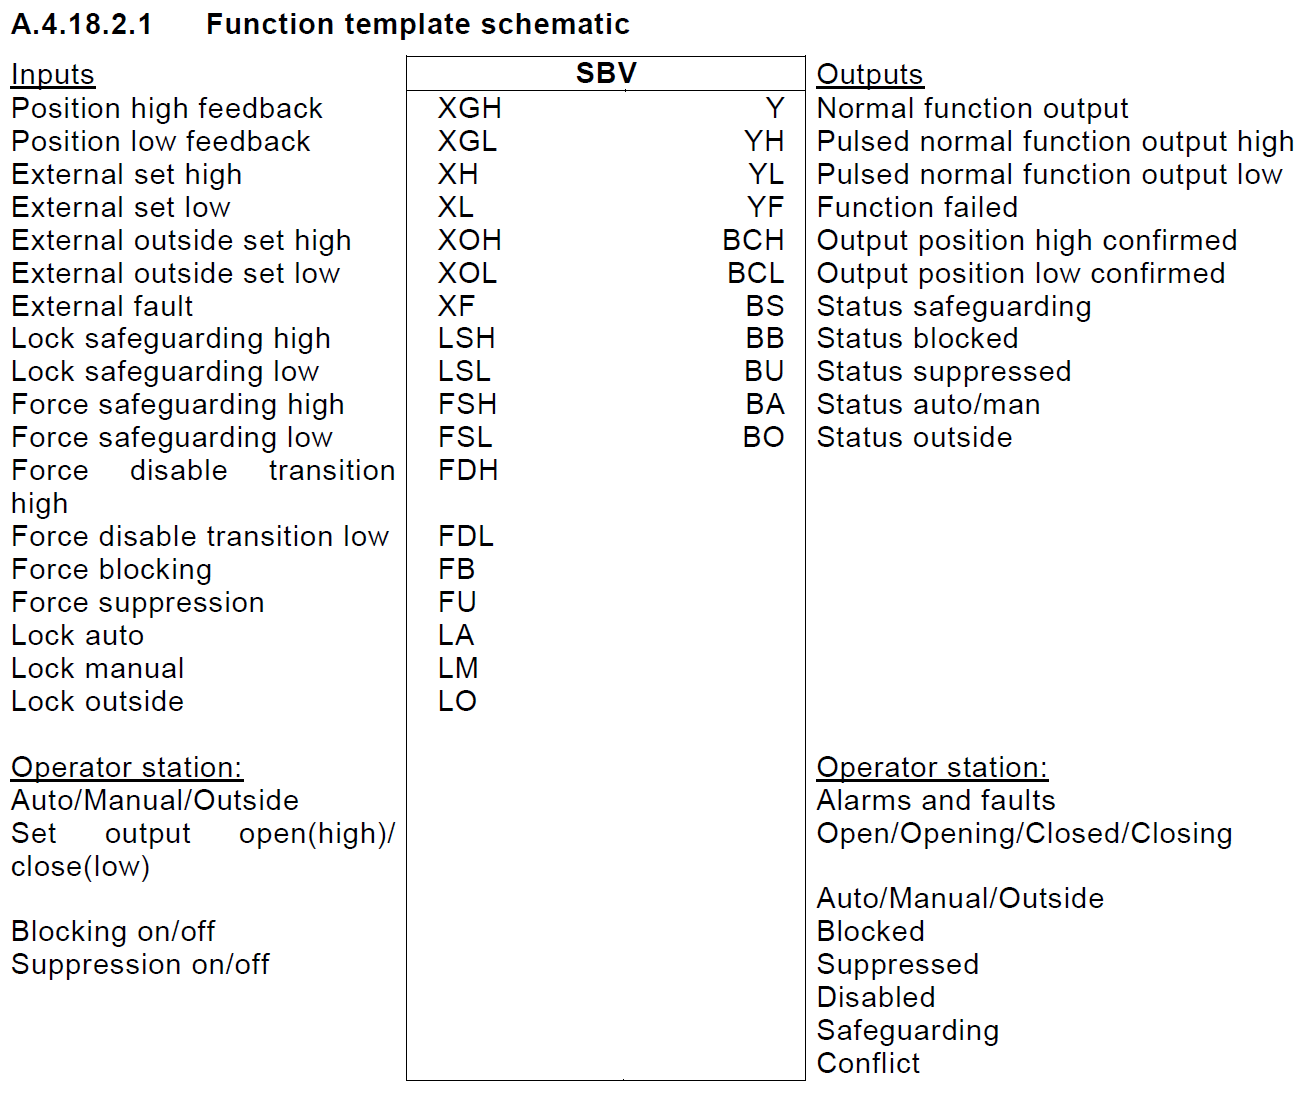
\includegraphics[width=1\textwidth]{Bilder/SBVBlokkIEC.png}
        \caption{IEC}\label{fig:Switch Binary Value blokk IEC}
    \end{subfigure}
    \hfill
    \begin{subfigure}[b]{0.45\textwidth}
        \centering
        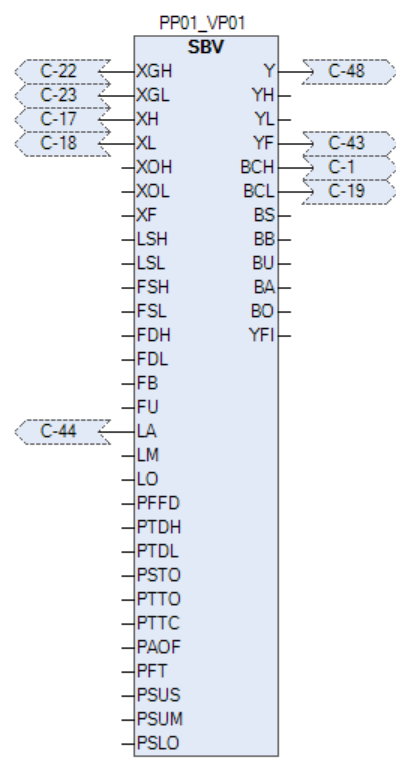
\includegraphics[width=0.5\textwidth]{Bilder/SBVBlokkIProgrammet.png}
        \caption{Bruk i programmet}\label{fig:Switch Binary Value blokk i programmet}
    \end{subfigure}
    \caption{Switch Binary Value}\label{fig:Switch Binary Value}
\end{figure}

\newpage

\subsection{Switch Binary Eletrical}

\gls{SBE} funksjonsblokka blir brukt for binærkontroll av straumningselement for elektrisitet, varme eller væske. Det
kontrollerte elementet er av typen motor, pumpe, varmeelement, vifte etc.

SBE blokka beskriver korleis ein kontrollarar ein enhet, for eksempel ein motor, pumpe, varmeelement, vifte etc.
Det er ein utgang Y, som gir ein opne/lukke (høg/lav) kommando til enheten. Blokka har fleire funksjonar, der den
tar output og samanliknar med tilbakemelding og gir korrekt BCL/BCH status. Den genererer også ein feil status på
YF om ein har ein ekstern feil inn.
Funksjonsblokka inkluderer alarm suppression, blocking, safeguarding og transition funksjonalitet.

\begin{figure}[htbp]
    \centering
    \begin{subfigure}[b]{0.45\textwidth}
        \centering
        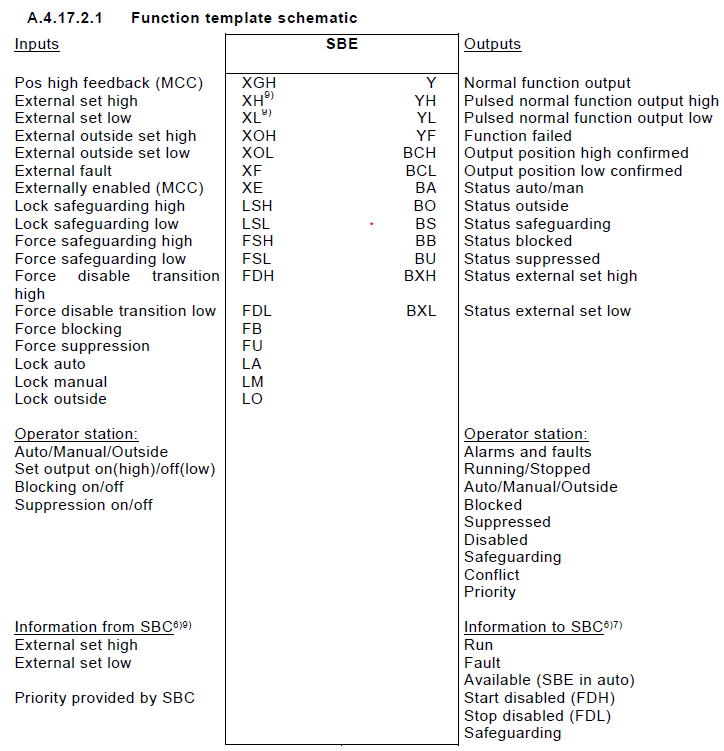
\includegraphics[width=1\textwidth]{Bilder/SBEBlokkIEC.png}
        \caption{IEC}\label{fig:Switch Binary Eletrical blokk IEC}
    \end{subfigure}
    \hfill
    \begin{subfigure}[b]{0.45\textwidth}
        \centering
        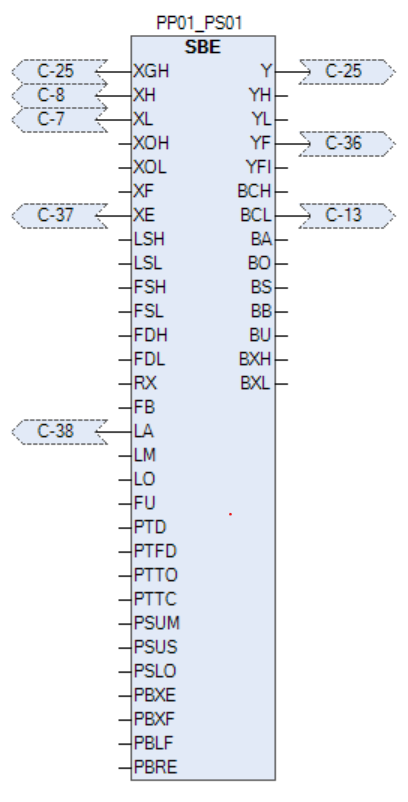
\includegraphics[width=0.5\textwidth]{Bilder/SBEBlokkIProgrammet.png}
        \caption{Bruk i programmet}\label{fig:Switch Binary Eletrical blokk i programmet}
    \end{subfigure}
    \caption{Switch Binary Eletrical}\label{fig:Switch Binary Eletrical}
\end{figure}

\newpage

%\begin{figure}[htbp]
%    \centering
%    \begin{subfigure}[b]{0.45\textwidth}
%        \centering
%        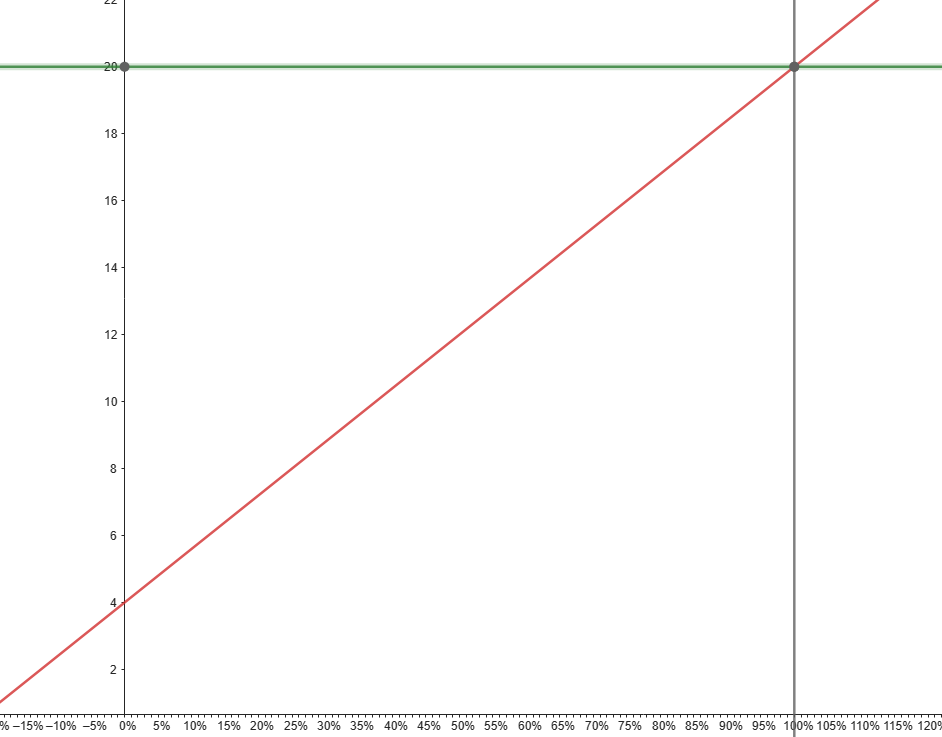
\includegraphics[width=1\textwidth]{Bilder/4_20mA_Scaling.png}
%        \caption{Skalering av mA mot prosent}\label{fig:Skalering av mA mot prosent}
%    \end{subfigure}
%    \hfill
%    \begin{subfigure}[b]{0.45\textwidth}
%        \centering
%        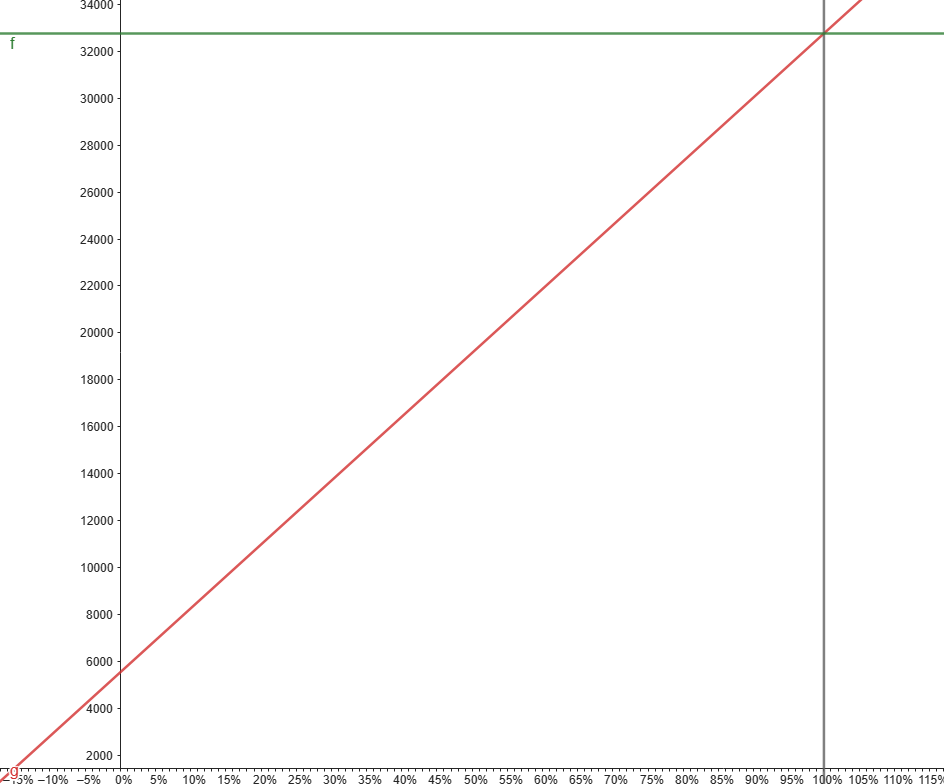
\includegraphics[width=0.95\textwidth]{Bilder/27327_prosent_Scaling.png}
%        \caption{Skalering av prosent til verdi}\label{fig:Skalering av prosent til verdi}
%    \end{subfigure}
%    \caption{Dei forskjellige skaleringane av inngangssignal}\label{fig:Skalering av prosent til verdi}
%\end{figure}


	\section{Tilstandsmaskin}
\thispagestyle{fancy}

\begin{figure}[htbp]
    \centering
    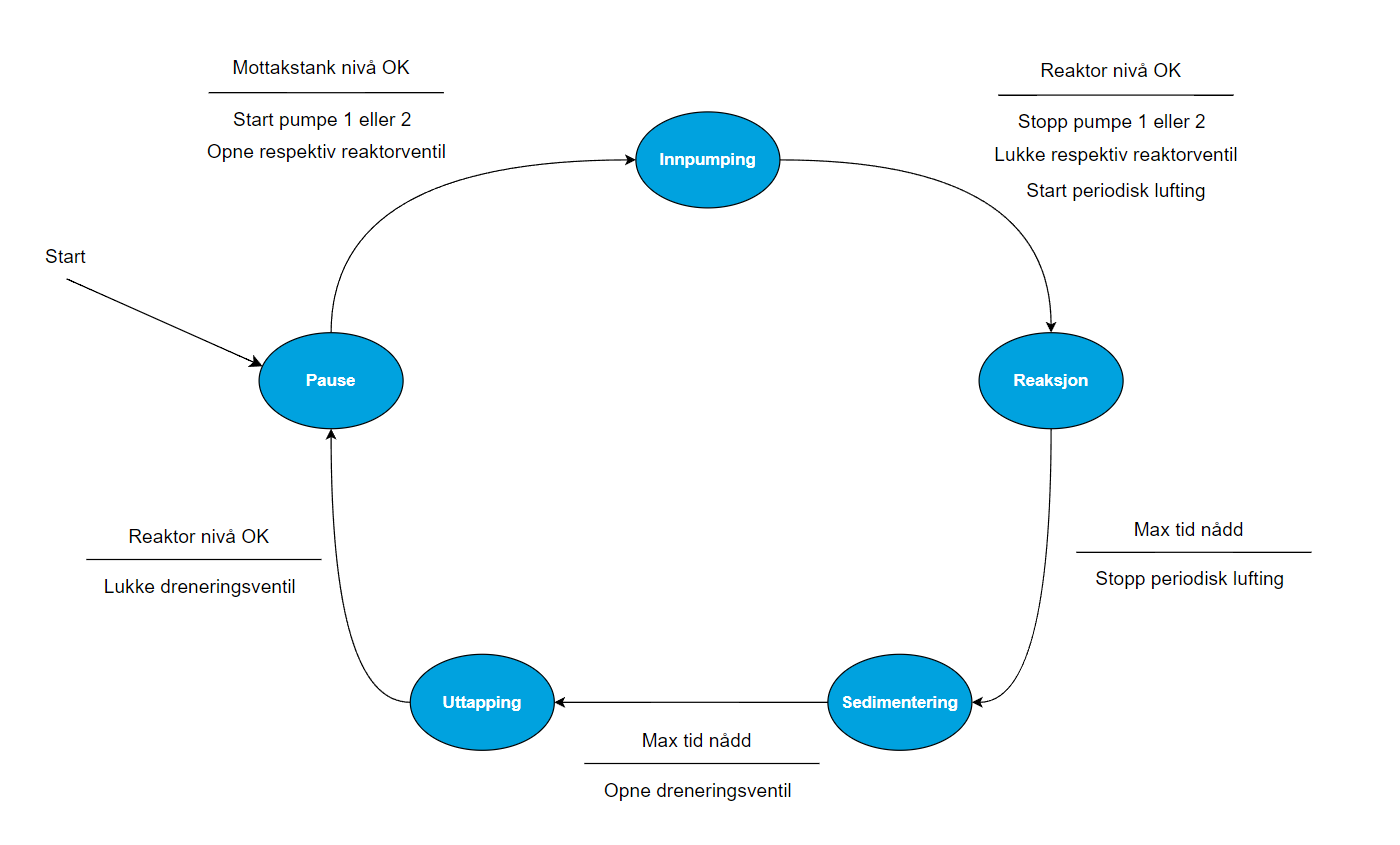
\includegraphics[width=1\textwidth]{Figurar/Simpel tilstandsmaskin.png}
    \caption{Simpel model av tilstandsmaskin}\label{fig:reaktorsoner}
\end{figure}


- Kjapt om programering av tilstandsblokka
	\newpage
\section{Tilstandslogikk}
\thispagestyle{fancy}

Styring og logikk som skulle skje i kvar tilstand valgte vi å samle i ei funksjonsblokk som fikk navn etter tilstanden
den skulle styre. Desse funksjonsblokkene er skrevet og løyst spesefikt for deira arbeidsoppgåver i programet og kvar
tilstand har eigen funksjonsblokk med tilstandslogikk. \newline
Kvar tilstandslogikk får inn XE (external enable) ifrå tilstandsmaskina som startar tilstandslogikken. Når sekvensen er ferdig sender
funksjonsblokka høg på utgang Y som returerast til tilstandsmaskina som avanserer til neste tilstand og tilstandslogikk.

Det er tilstandslogikken som har ansvar for å samarbeide med IEC-blokkene som vidare
leser inngangssignal, startar og stoppar elektrisk utstyr, kontrollerer feedback, feilmeldingar og skriv akutelle parameter.

\begin{figure}[htbp]
    \centering
    \begin{subfigure}[b]{0.3\textwidth}
        \centering
        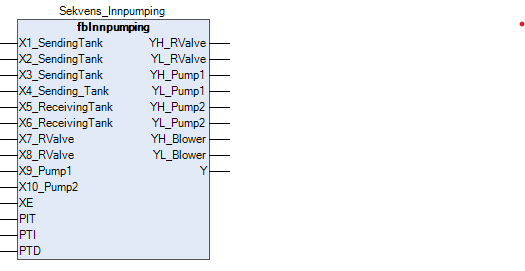
\includegraphics[width=1\textwidth]{Bilder/fbInnpumping.png}
        \caption{Innpumping}\label{fig:subfig1}
    \end{subfigure}
    \hfill
    \begin{subfigure}[b]{0.3\textwidth}
        \centering
        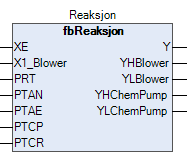
\includegraphics[width=1\textwidth]{Bilder/fbReaksjon.png}
        \caption{Reaksjon}\label{fig:subfig2}
    \end{subfigure}
    \caption{Utklipp av tilstandslogikk}\label{fig:Illustrasjon-Diffuser}
\end{figure}




	\newpage
\section{Oppbygging av programmet}
\thispagestyle{fancy}

\subsection{Programmeringsmetode}
For å sette i sammen alle funksjonsblokkene, som vi hadde skreve i strukturert tekst, valgte vi å bruke \GLS{Codesys} CFC.
CFC (Continuous Function Chart) er er ein grafisk programmeringsmetode som bruker symbol og koplingar for å gjere programmet  meir visuelt.

Alle sammensettningar av blokker valgte vi å gjere i CFC. Ved å bruke ein grafisk metode sikra vi oss god lesbarhet og
visuell forståelse i programmet. 

Alle inngangar og utgangar er leselige og enkle og forstå. CFC ilag med god dokumentasjon vil kunne gi personar utan programmeringsbakgrunn
god forståelse av korleis programmet er satt opp, utan å måtte lese linjer med kode.
CFC gir godt grunnlag for feilsøking og analyse og bygger derfor vidare på filosofien med eit enkel og fleksibelt program.

Dersom antall koplingar og linjer gjorde programmet vanskeleg å lese var det også
mogleg å opprette `source' og `links' som oppretta ein trådlaus forbindelsane gjennom ein unik ID.


\begin{figure}[htbp]
    \centering
    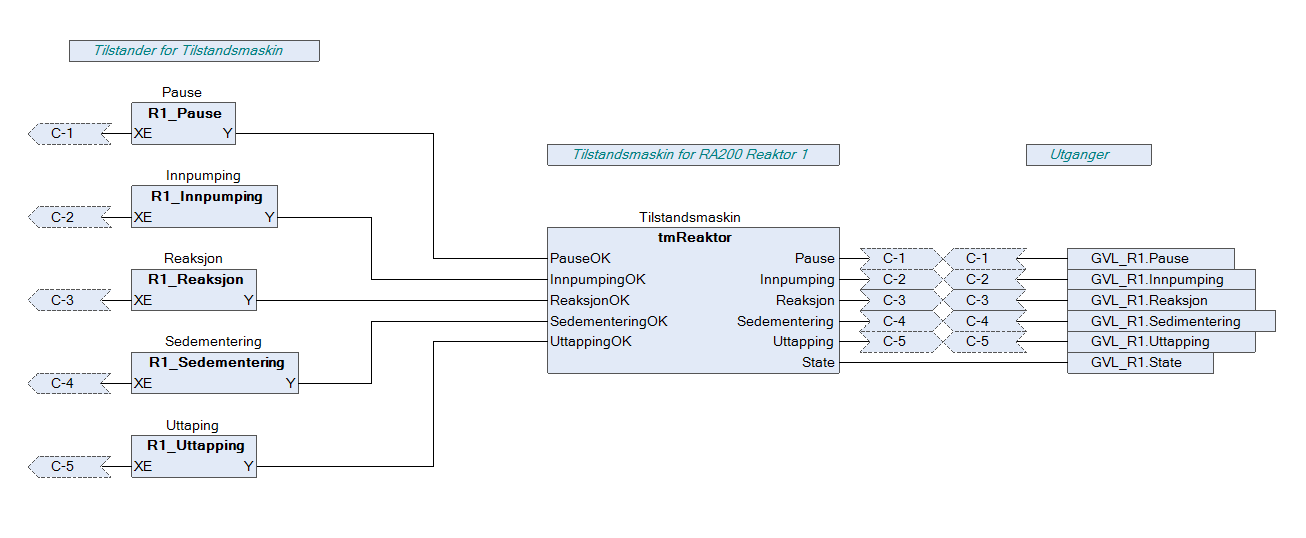
\includegraphics[width=1\textwidth]{Bilder/ReaktorPRG.png}
    \caption{Eksempel CFC - Styring reaktor 1}\label{fig:reaktorsoner}
\end{figure}

\newpage

\subsection{Hovuddel}

Programmet er delt opp i tre hovuddelar, ei tilstandsmaskin for kvar reaktor og ein del for samling av felles reaktor funksjonar.
Alle desse har eit kall i MainTask og blir utført kvar PLS syklus. Tilstandsmaskina har overordna ansvar og bytter på kva 
\gls{FB} med tilstandslogikk som køyrer.

Felles funksjonar er ein samling av funksjonsblokker og utrekningar som er felles og eller uavhengig av reaktorane med tilstandsmaskin.
Driftsovervåking er ein sentral del av felles funksjoner, der timetelling og mengde prosessert vatn er eksempel på funksjonar og utrekningar
som blir gjennomført.

I enkelte tilfeller måtte, som ved rullering av sivbed, var vi avhengig av at både tilstandsmaskin for reaktor 1 og reaktor 2 hadde samme informasjonen.
Dette løyste vi ved å lage ei fbSivbedRotation i felles funsjonar som henter inn og akummulerte antall slamutakk for så å rotere når ei git grense var nådd.
Denne informasjonen blir så sendt til kvar tilstandsmaskin og sørger for at begge reaktorane har same aktive sivbed.


\begin{figure}[htbp]
    \centering
    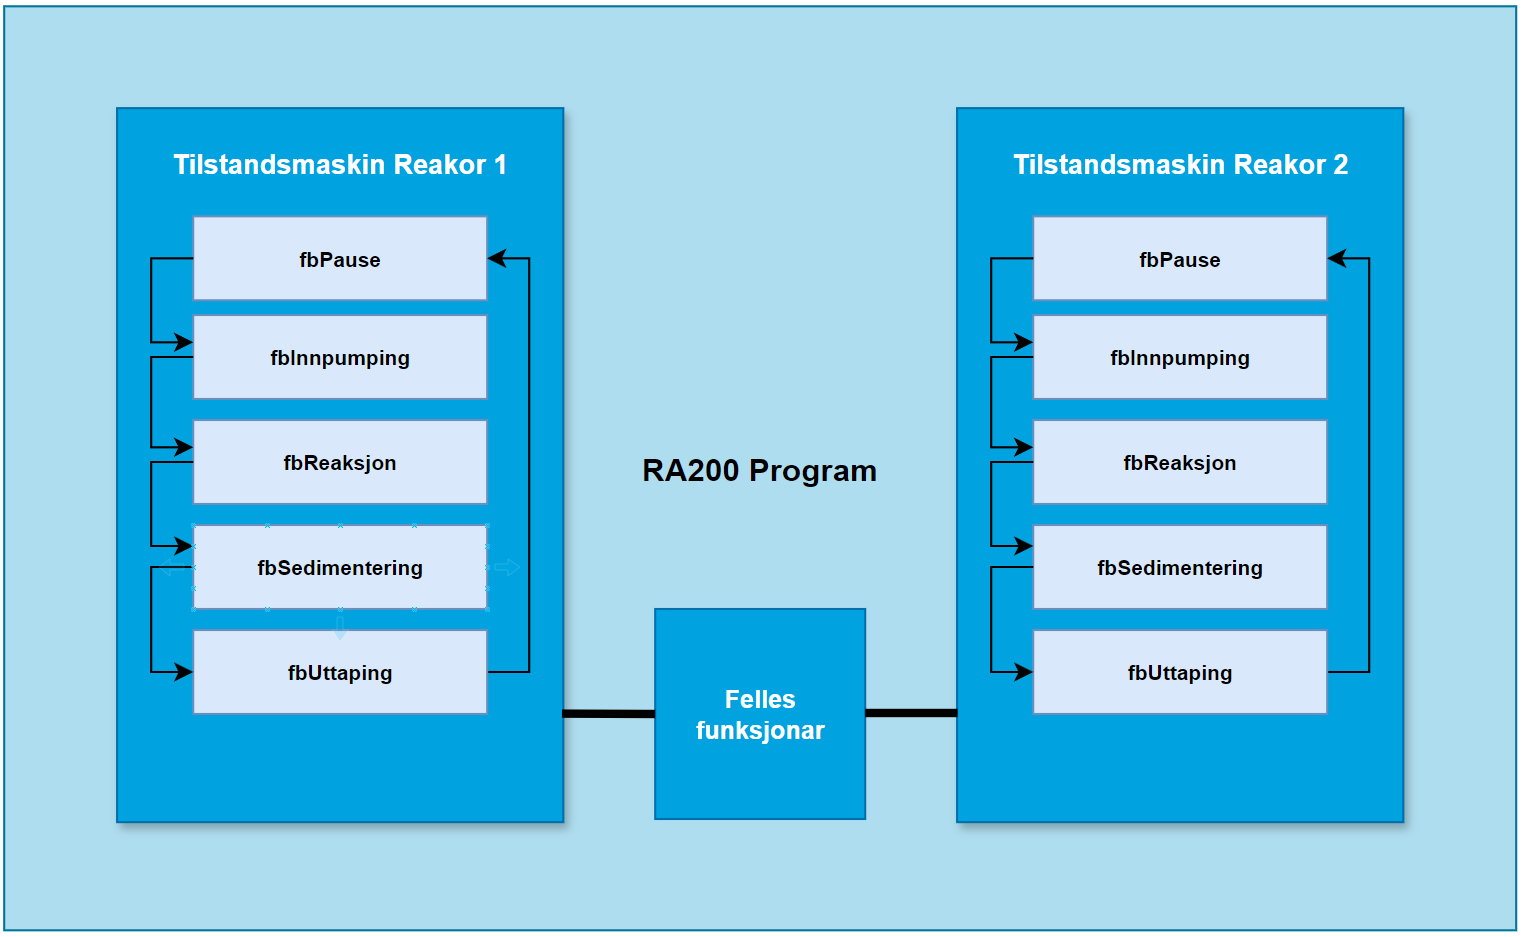
\includegraphics[width=1\textwidth]{Figurar/Oppbygging_Program.png}
    \caption{Illustrasjon oppbygging av programmet}\label{fig:reaktorsoner}
\end{figure}


\newpage

\subsection{Styring tilstandslogikk}

Som nemnt tilegare er det tilstandslogikken som samarbeider opp mot IEC blokkene. Dette samarbeidet valge vi også å gjere i eit
CFC vindu som igjen gjorde kall og koplingar visuelle. Dette CFC vinduet fikk navn etter kva sekvens i SBR-prosessen
den hadde ansvar for å styre. 

Oppbyggningen av desse sekvensstyringane er gjort med inngangsblokker (MA og MB) øvst og utgangsblokker (SBE og SBV) i bunn.
I mellom desse kjem sjølve tilstandslogikk blokkene som inneholder sjølve logikken.

\begin{figure}[htbp]
    \centering
    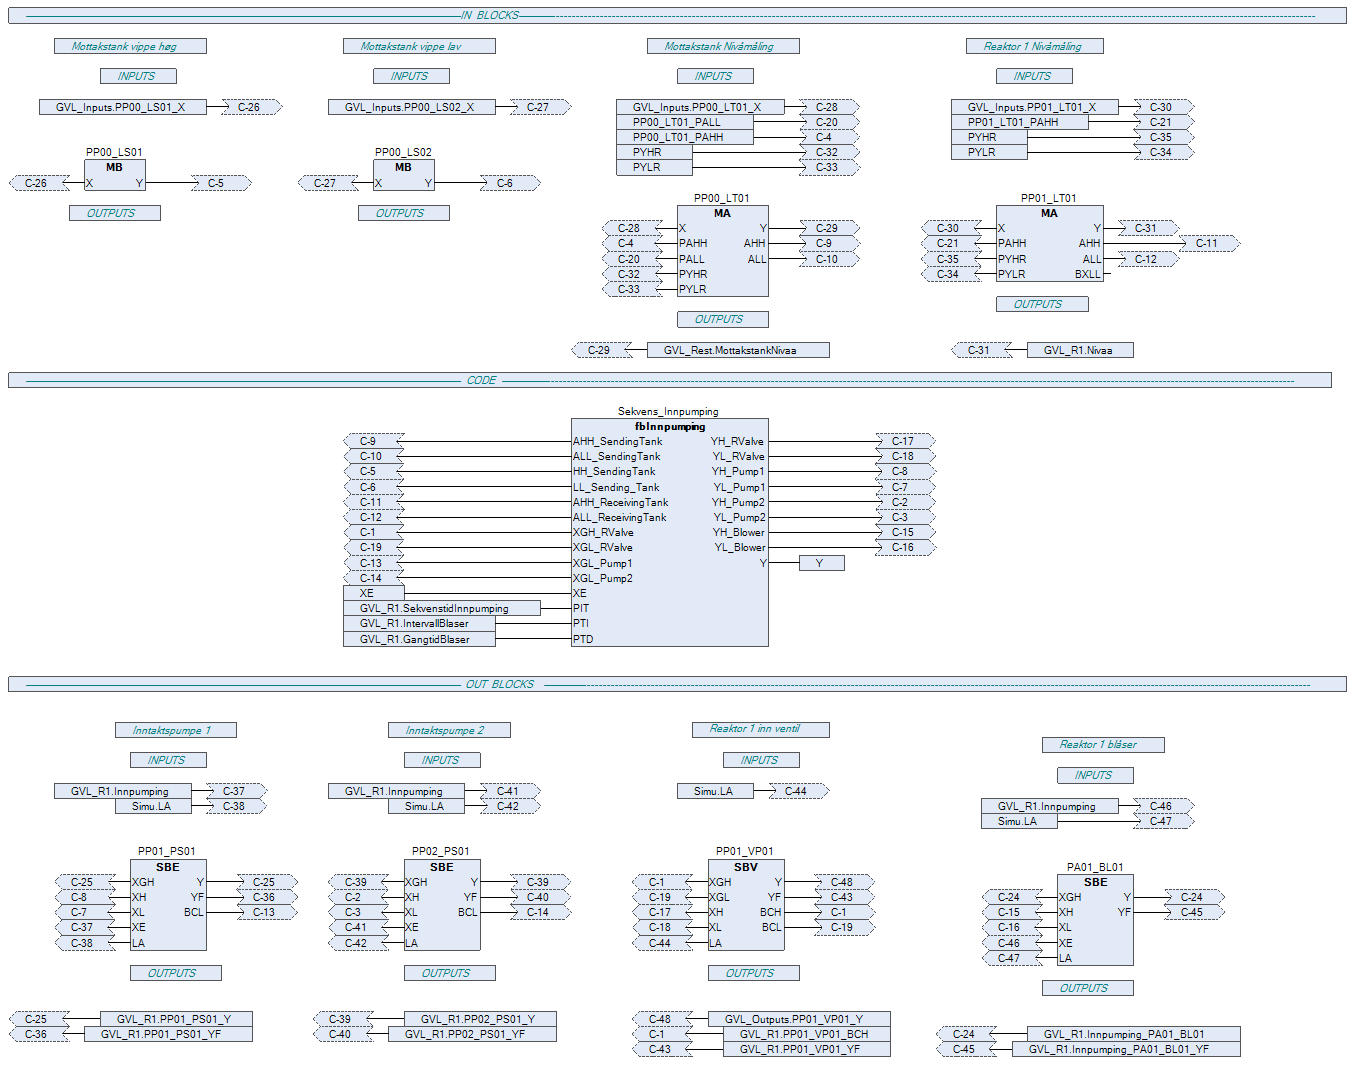
\includegraphics[width=1\textwidth]{Bilder/Heile_innpump.png}
    \caption{Eksempel CFC - Styring Innpumping}\label{fig:reaktorsoner}
\end{figure}

I denne figuren er ekstra inngangar, parameter inngangar og ekstra utgangar fjerna for å bedre visualisere kopllinga og samarbeidet mellom
IEC blokkene og funksjonsblokk for tilstandslogikk.

\newpage


	\section{Utfordringer}
\thispagestyle{fancy}

Vi opplevde noko problematikk rundt det å ha fleire blokker, som styrer samme komponentar da vi skrivar til ein felles global variabel.
Denne variabelen blir då satt true og false i frå fleire plassar i programmet, noko som gjer at variablenen sinn tilstand vil vere tilfeldig, basert på korleis Codesys sin kompilator leser koden.

Dette kan vi løyse ved å bruke ein egen global variabel for kvar blokk, og så skrive til ein funksjonsblokk som styrar den endelege globale variabelen.
Det er fleire plassar i programmet vi møter denne utfordringa, som blant anna med pumpestyring, da kvar reaktor kan styre same pumpe.
Same løysning vil gjelde i denne situasjonen, der vi må lage ei blokk som tar inngangar frå begge pumpene og setter utgangen til riktig tilstand.  

Dette er eit klassisk eksempel der vi har koda noko vi trur fungera optimalt, men under testing så finner vi ut at det ikkje fungera som vi har tenkt.
Løysninga setter nokre føringar for variabelhandtering videre i programmet, og vi står over eit val der valet våra gjer koden noko meir avansert, men vi oppretthelder funksjonaliteten i programmet slik vi opphavleg hadde tenkt.


	% Kapittel 7 Dokumentasjon
	\chapter{Tillrettelegging for programmering}
\thispagestyle{fancy}
\label{sec:7} 

Som tidlegare beskrevet under kapittel \ref{sec: 5}, ynskte vi å bruke ei løysning som ikkje hadde høge lisenskostnadar for vår sluttkunde. 
Sunnfjord kommune var interessert å ikkje låse seg til ein fast leverandør, men heller ha moglegheita til å ha valet mellom fleire 
leverandørar innan \gls{PLS}. Dette ilag med moglegheiten til å utivde vår eigen kompetanse 
gjorde at vi såg vekk ifrå Siemens \gls{TIA}-portal \citep{Siemens}, som vi hadde lært igjennom \gls{PLS} emnet.
Programmet ynskte vi å skrive i strukturert tekst (\gls{ST}) men undersøkte også 
typar av grafiske diagrambaserte språk for å lettare vise samanhengar i programmet.

Det var også viktig at alle på gruppa kunne programmere samtidig og at ein felles programmeringsstandard skulle nyttast.
Det var viktig at parallelt arbeid ikkje skulle by på synkroniserings problem og at det fantest ei god løysning for dette.


	\section{Alarmliste}
\thispagestyle{fancy}

Alarmliste, cause og effect
elefanten
\citep{website}
	\section{Interlock}
\thispagestyle{fancy}

Det er nytta «interlock» av funksjonar nokre plassar i programmet. 
Sidan vi brukar IEC blokkar til styring av alle våra objekt, har vi funksjonalitet i blokkene som gjer det enkelt for oss å handheve forriglingar mellom komponentar. I tillegg har vi overordna kontroll med at tilstandsmaskina gir signal til XE, slik at dei komponentane som ikkje er i bruk i sekvensen, skal ikkje kunne vere tilgjengeleg.

Objekter som krever forriglingar:

Sett inn tabell/bilde over forriglinger, kva forigla mot, korleis.

Pumpe 1,Pumpe 2, Innpumpingssekvensane, ventilar
	
	\section{IO-liste}
\thispagestyle{fancy}

Når det kommer til \gls{IO} liste, så har vi ikkje noko konkret å visa til, sidan våra løysningsforslag baserer seg på ein teoretisk løysning. 
Vi har difor tatt utgangspunkt i ein minimum I/O som allereie ligger til stades i frå det tidlegare anlegget (sjå Appendix \ref{sec:IOliste}). 
I tillegg så har vi laget til moglegheit for fleire inngangar basert på ønsket tilleggsmål gitt av arbeidsgivar. 
Dette er inngangar som til dømes tilbakemelding av ventilar, flowmåler og temperaturgivera.
Dette er inngangar som er veldig enkle å legge til i ettertid, da programmet er bygget opp med dette i tankane.
	\section{Objektliste}
\thispagestyle{fancy}


	\section{P-ID}
\thispagestyle{fancy}

Kan kanskje mergest i lag med scd-diagram at det er egen section med kanskje under sections
	\section{Vedlikeholdsmanual}
\thispagestyle{fancy}

Alarmliste, cause & effect
	\section{SCD-Diagram}
\thispagestyle{fancy}

Må lage til og legge inn SCD v1 og SCD v2 - ferdig versjon.

	% Kapittel 8 Simulering og verifisering
	\chapter{Simulering og verifisering}
\thispagestyle{fancy}

Forklare prossessen med simulering av anlegget. Korleis vi har laga simuleringsverktøyet, simuleringsprossessen i Codesys, osv
	\section{Kontinuerlig simulering}
\thispagestyle{fancy}

Undervegs i programmeringa har vi gjort kontinuerlege testar og simulering av blokkene vi har laga og
har vært ein sentral del av arbeidsmetodane vi har brukt i prosjektet. 

Kontinuerleg simulasjon er smø øvingar og tester som ein utfører medan ein arbeider.
Det er ikkje ein testfase med klare start og stopp, men små kontinuerlege testar og sjekkar som gir tilbakemelding
om arbeidet ein har utført følger spesifikasjonane.

I dette prosjektet brukte vi mykje kontinuerleg simulasjon i programmering av IEC blokkene.
Desse blokkene hadde mange funkjonaliteter som ikkje nødvendigvis var avhengig av kvarandre og
det medførte at vi kunne gjere små enkle testar på dei forskjellege områda uten at heile blokka var ferdig. \newline
Som eit eksempel skal RX resete ein utgang Y. Dette blir implimentert og deretter testa ved hjep av simulasjon.
Kva som til slutt skal sette utgang Y høg er ikkje relevant i dette tilfellet, men vi har implimentert 
og testa at ein reset vil fungere.

\newpage
	\section{Simulerings blokker}
\thispagestyle{fancy}


For å skape eit meir realistisk miljø for testinga lagde vi nokre simuleringsblokker.
Desse blokkene etterlignar driftssitasjonar og gjer simuleringa enklare og betre.
Vi lagde i hovudsak to slike blokker, ei blokk som simulerer fylling av ein tank
og ei blokk som simulerer tilbakemelding frå ventilar.

Blokk for tank simulering er enkel og skreven spesfikt for Sande reiseanlegg med ein mottakstank
og to reaktorar.
Det er usansyneleg at desse simuleringsblokkene vil bli brukt vidare, men dei gav
oss den realismen vi trengte.

Blokkene er også med å gjere sjølve arbeidet med simuleringa enklare.
Før vi lage blokk for tilbakemelding på ventilar, 
gav vi manuelt kvar ventil XGH eller XHL basert på kor den eigentleg skulle være (open/lukka).
Dette fungerer greit dersom ein tester små områder eller kun ein ventilblokk, men
når ein simulerer ein større grad av programmet blir denne jobben tidkrevjande.

På desse blokkene har vi tatt oss meir friheit i namngiving, feilhandtering osv
fordi blokkene ikkje skal brukast når programmet er ferdig.

\begin{figure}[htbp]
    \centering
    \begin{subfigure}[b]{0.3\textwidth}
        \centering
        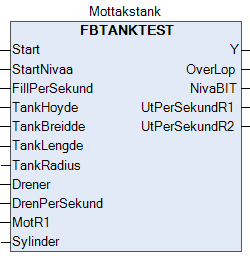
\includegraphics[width=0.9\textwidth]{Figurar/TankSim.png}
        \caption{Tank}\label{fig:subfig1}
    \end{subfigure}
    \hfill
    \begin{subfigure}[b]{0.3\textwidth}
        \centering
        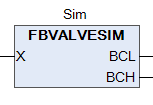
\includegraphics[width=0.9\textwidth]{Figurar/ValveSim.png}
        \caption{Ventil}\label{fig:subfig2}
    \end{subfigure}
    \caption{Simuleringsblokker}\label{fig:Illustrasjon-Diffuser}
\end{figure}

\newpage
	\section{Full simulasjon}
\thispagestyle{fancy}

Skriv litt om fullstending simmulering av anlegget.
Legg ved screenshot av simuleringsvinduet menst vi køyrer simulering på begge reaktorar

	% Kapittel 9 Diskusjon
	\chapter{Diskusjon}
\thispagestyle{fancy}
Her kan vi starte underlaget for kappittelet
	\section{Vegen videre for anlegget og programmet}
\thispagestyle{fancy}

Sida oppgåva er ein teoretisk løysningsforslag på eit nytt PLS program i frå reinseanlegget på Sande, er det nokre praktiske detaljar som dukkar opp.

\begin{itemize}
    \item Manglar å mappe fysiske inn og utgangar
    \item Gammalt program nyttar ASiMASTER-bus  
    \item Utviding av det eksisterande anlegget med ny teknologi frå Renasys
    \item Manglande gjennomstrøymingsmåler.
\end{itemize}

Da vi forventar at anlegget går igjennom ein større ombygging,  da med tanke på Renasys og Kommunen sin dialog om utviding av det eksisterande anlegget med ny Renasys teknologi, er dette noko som bør vurderast opp mot programmet og om det blir behov for å endre eller legge til noko. 
Dette er eit naturleg punkt å vurdere tilleggsmåla, om dei ønsker å implementere noko av desse.
Det gamle programmet brukar i dag ASiMASTER-bus for tilkopling av ein del av komponentane mot PLS. 
Dette er noko eigar av anlegget må ta stilling til om ein ønsker å fortsette med eller gjere om. Alle dei fleste ventilar er styrt over bus, og om ein ønskjer å bruke ventilar med tilbakemelding på opne og lukke signal, må det nokre ombyggingar til sidan det berre er laga til for utgangar frå PLS ved ventilane.
Styreskapet der den gamle PLS står i, har då noko redusert plass om ein byrjar å utvide anlegget med fleire modular. 
Dette er moment som må takast med videre om ein ønsker å oppgradera anlegget. 



	\section{Vegen vidare for programmet}
\thispagestyle{fancy}


Sida oppgåva er ein teoretisk løysningsforslag på eit nytt PLS program (SKRIVAST OM?), så er det nokre praktiske moment som oppgåva ikkje reflektera.
Programmet 


\begin{itemize}
    \item Manglar å mappe fysiske inn og utgangar
    \item Gammalt program nyttar ASIMASTER-bus
    \item 
    \item   
\end{itemize}

	% I henhold til forrapporten skal vi og ha elektriske teikningar, brukarrettleiing og vedlikehaldsmanual
	
	% Kapittel 10 Konklusjon
	\chapter{Konklusjon}
\thispagestyle{fancy}
Må skrivast i fortid
	\chapter{Avslutting}
\thispagestyle{fancy}
Og så avslutta vi alt, og det var fint vær og konge.

    
	\chapter{Konklusjon}
\thispagestyle{fancy}
Vi ønsker å gjere godt eit arbeid. Dette medfører at vi ønsker å ta for oss ein mindre del av prosessen for å løyse oppgåva på best mogleg måte.
 Alternativet er å ta ein større del t.d. programmering i tillegg til installasjon.
  Men med avgrensa tid kan dette medføre at arbeidet ikkje når potensialet vi ønsker.

Oppgåva vil bli løyst kunn teoretisk sjølv om anlegget er fysisk. 
Ved ei teoretisk oppgåva kan vi legge vekk noko av fokuset på sikkerhetsmomenta ved ein ny installasjon,
og heller bruke meir tid på sikker og robust programmering ilag med ein komplett og korrekt dokumentasjonspakke.

Løysningsalternativ to er det alternativet som blir best for oss. 
Anlegget har manglande dokumentasjon, 
og mykje av arbeidet vil være å bygge ein god funksjonsbeskrivelse for å gjere vidare programmeringsarbeid med reinseanlegget enklare.
	\section{Exit Points}
\thispagestyle{fancy}
(Denne kan kanskje flyttes til kap3)
Vi har definert nokon praktiske punkt i oppgåva der vi har moglegheit 
for å naturleg å avslutte arbeidet om ein ser at vi ikkje får nok tid,
eller at vi har tid til overs. 
Det originale stop punktet vårast er definert etter kravspesifikasjonen. Naturleg alternativ stopp punkt.

\begin{itemize}
    \item Etter programmering og før simulering og verifikasjon
    \item Før programmering.
\end{itemize}

Ved ekstra tid, har vi disse tilleggsoppgåver frå arbeidsgivar 
som kan implementerast i den nye styringssystemet.

Undersøke forbetringspotensiale av anlegget:
\begin{itemize}
    \item Temperatursensor
    \item Nivåsensor
    \item Trykksensor (reintvann inn)
    \item Ventiltilbakemeldingar
    \item Oksygenmåling
    \item Mengde måling «overflow»
    \item Frekvensstyring på hovudpumper
    \item Integrere MJK prøvetakar
    \item Energimåling
\end{itemize}

	\clearpage
	\renewcommand{\glossaryname}{Ordliste} % Denne er med for å kunne endre navn på ordlista
	\printglossaries %Printer ut alle ord som er brukt frå ordlista

	%Referanseliste (Berre for test, citep må flyttast inn i teksten)
	%\clearpage
	%\chapter{Referansar} % sjekk om det skal være slik, for å få den opp i innhaldslista.
	\clearpage
	\bibliography{Referansar} % Dette er ein referanse til Referansar.bib
	\addcontentsline{toc}{chapter}{Referansar}  % Adds the unnumbered chapter to the table of contents


	% Create a partial table of contents for appendices
	% Generate the list of appendices
	% Start of appendices, capture contents for appendices list
	%\begin{appendices}
	%	% This command initializes the recording of contents for appendices
	%	\startcontents[appendices]
	%	\phantomsection
	%	\addcontentsline{toc}{chapter}{Liste av Appendikser} % Her kan ein endre navn for appendix lista
	%	%\chapter{MB Blokk}
%Dette er ein appendiks for MB blokka
%\includepdf[pages=-]{MB Dokumentasjon.pdf}  

\chapter{IEC Blokker}

% MB Blokk
% Include only the first page
\includepdf[pages=1,scale=0.8, pagecommand={\section{Montor binary}\thispagestyle{empty}},fitpaper=true]{Appendix/IEC Blokker/MB Dokumentasjon.pdf}
% Include the rest of the pages, Starts from the second page to the last, Keep the same scale for all pages
\includepdf[pages=2-, scale=0.8, pagecommand={\thispagestyle{empty}}, fitpaper=true]{Appendix/IEC Blokker/MB Dokumentasjon.pdf}

% MA Blokk
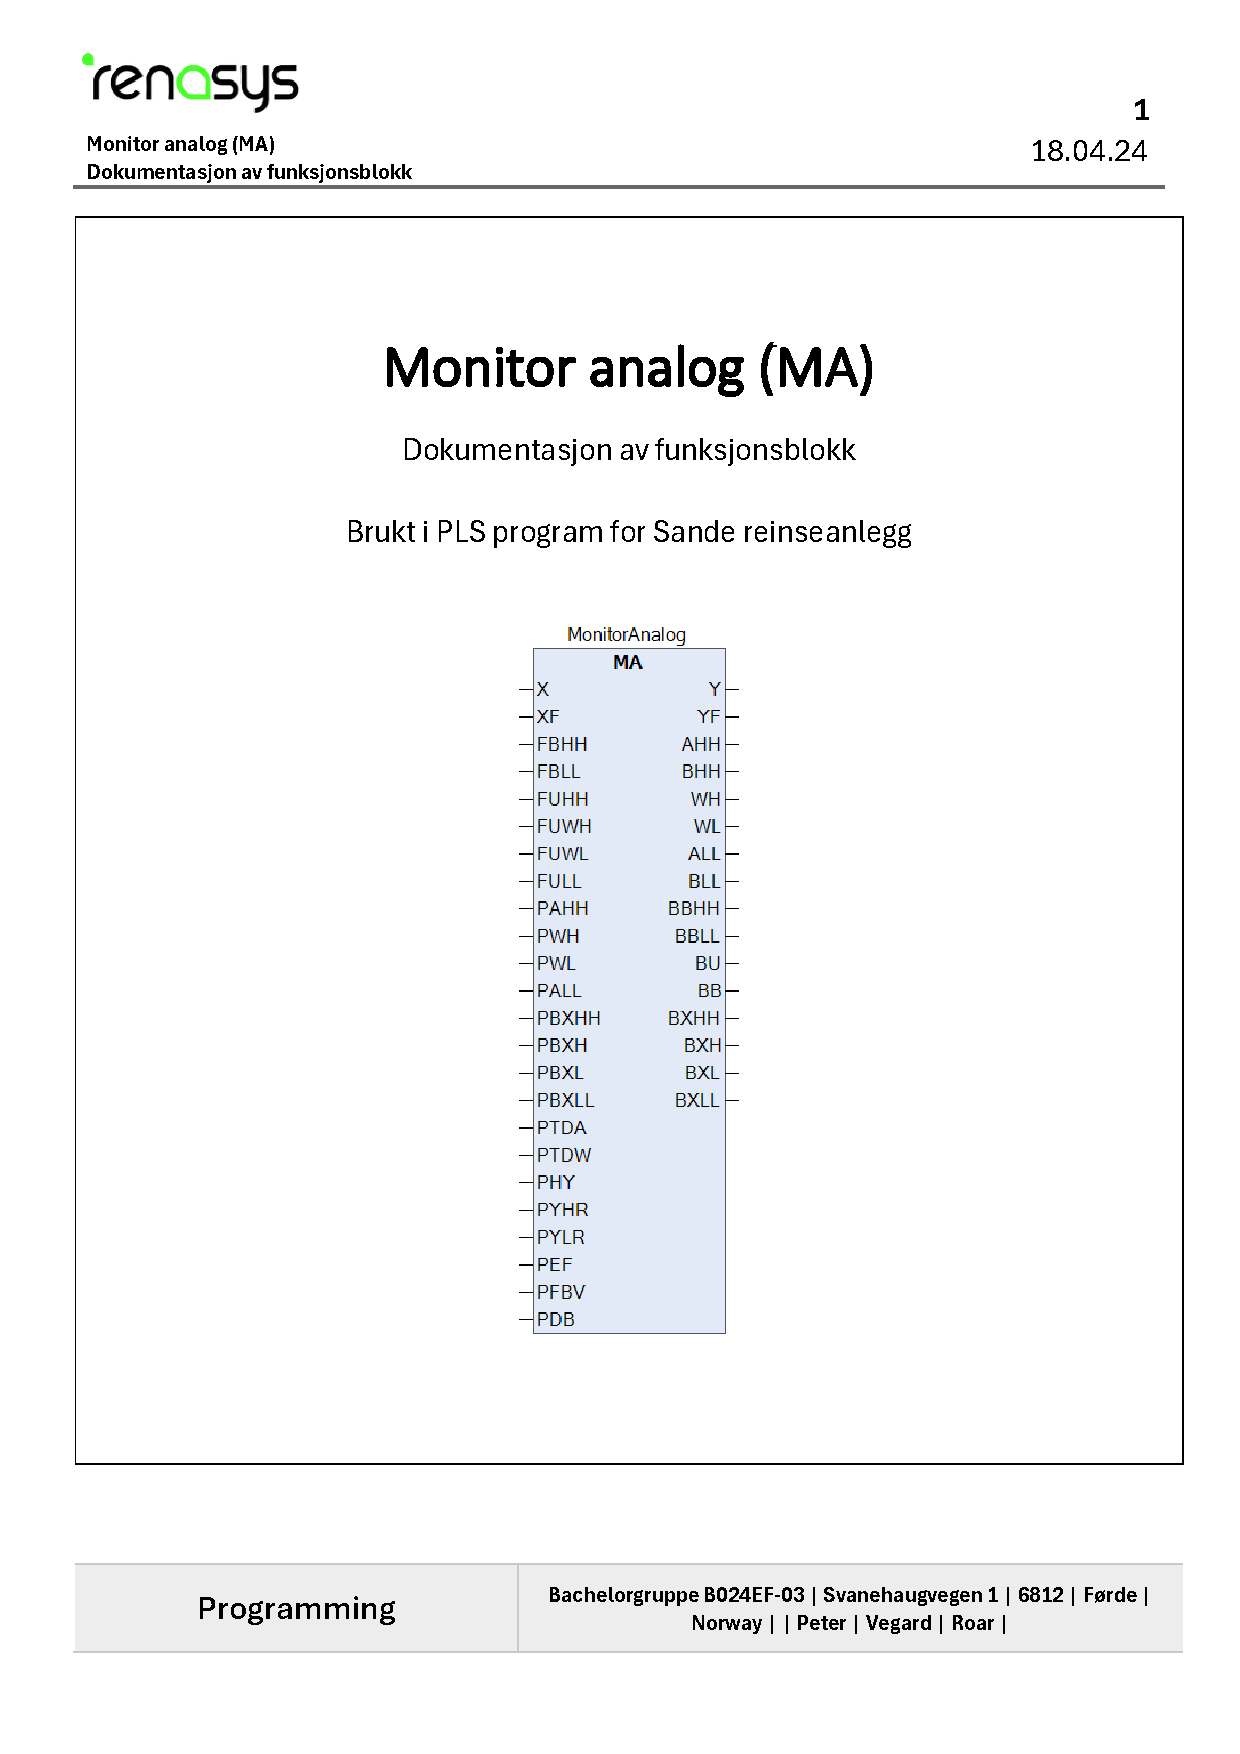
\includepdf[pages=1, scale=0.8, pagecommand={\section{Monitor Analogue}\thispagestyle{empty}}, fitpaper=true ]{Appendix/IEC Blokker/MA Dokumentasjon.pdf}
\includepdf[pages=2-,scale=0.8, pagecommand={\thispagestyle{empty}},fitpaper=true]{Appendix/IEC Blokker/MA Dokumentasjon.pdf}

% SBE Blokk
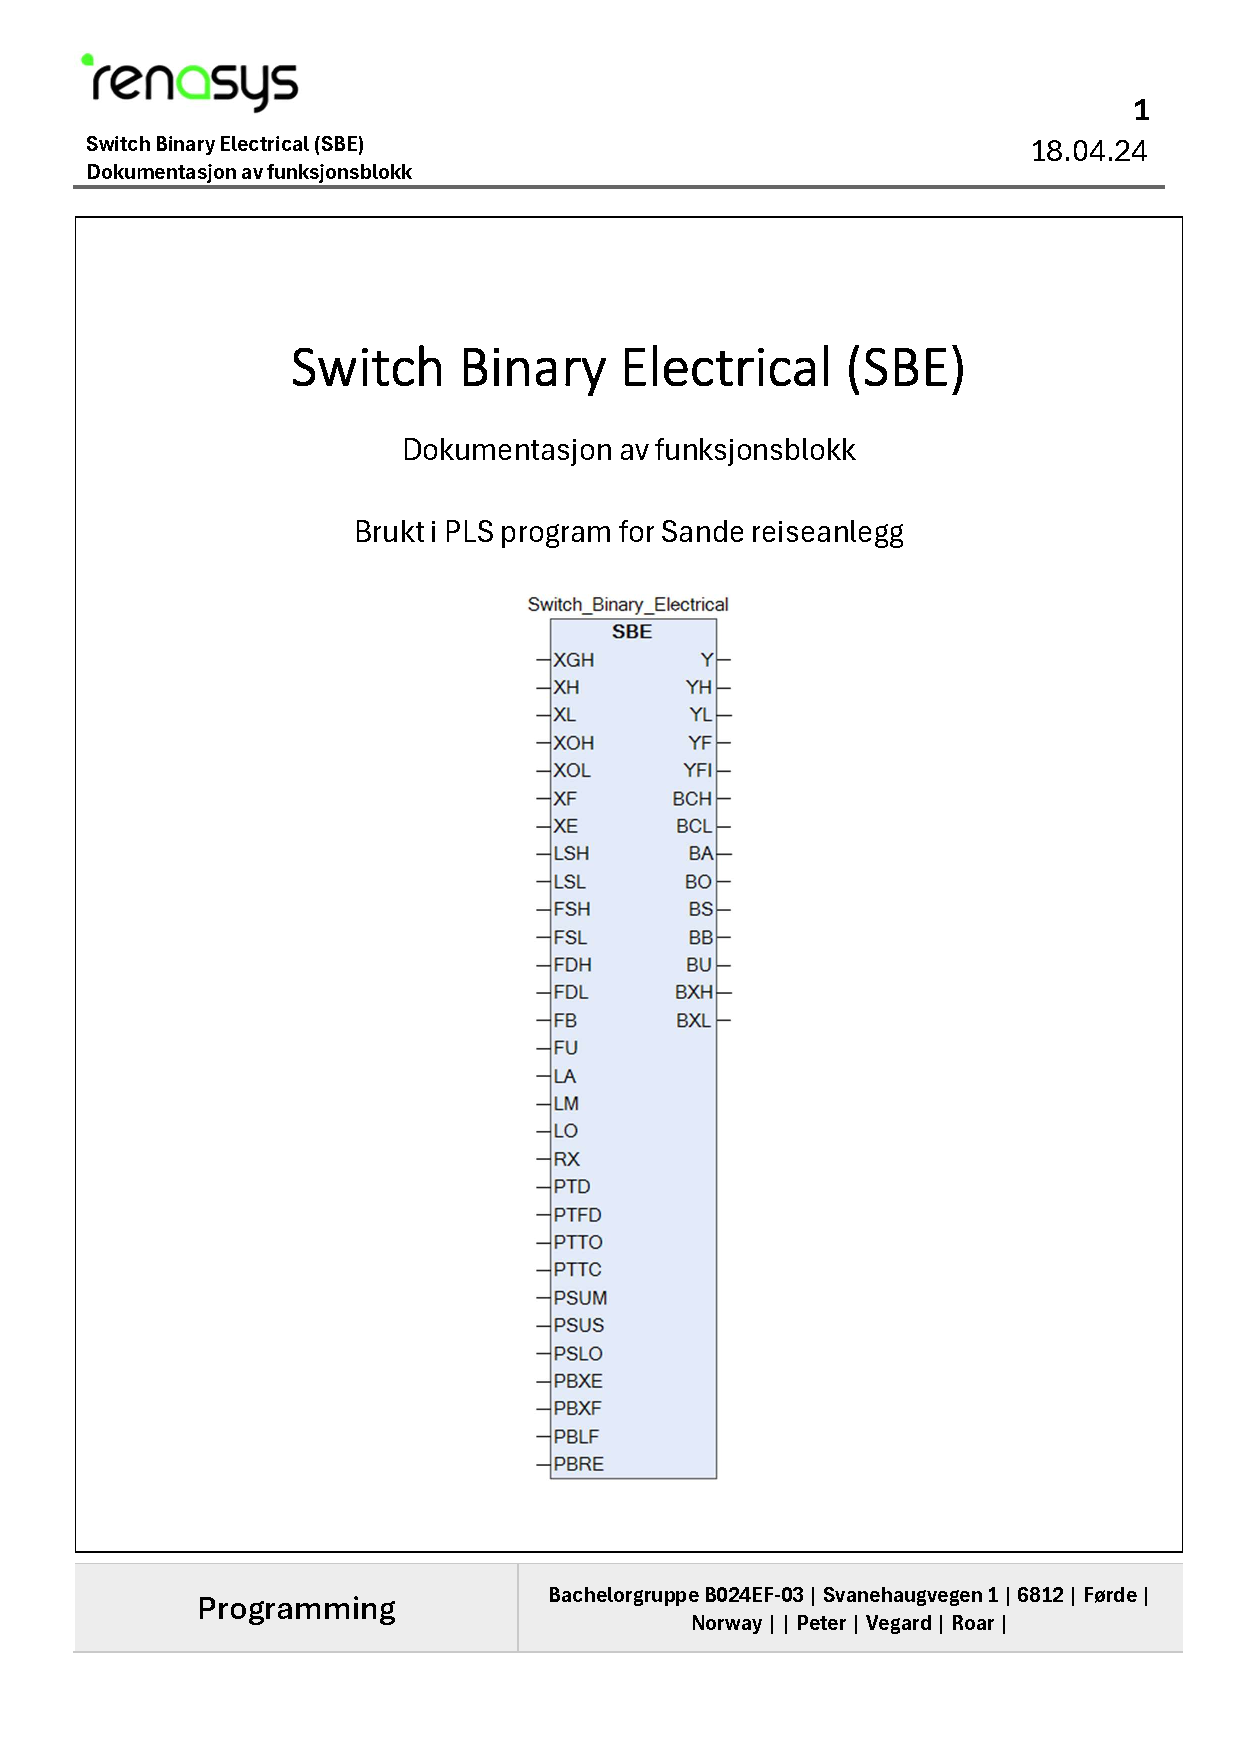
\includepdf[pages=1, scale=0.8, pagecommand={\section{Switch Binary Eletrical}\thispagestyle{empty}}, fitpaper=true ]{Appendix/IEC Blokker/SBE Dokumentasjon.pdf}
\includepdf[pages=2-,scale=0.8, pagecommand={\thispagestyle{empty}},fitpaper=true]{Appendix/IEC Blokker/SBE Dokumentasjon.pdf}

% SBV Blokk
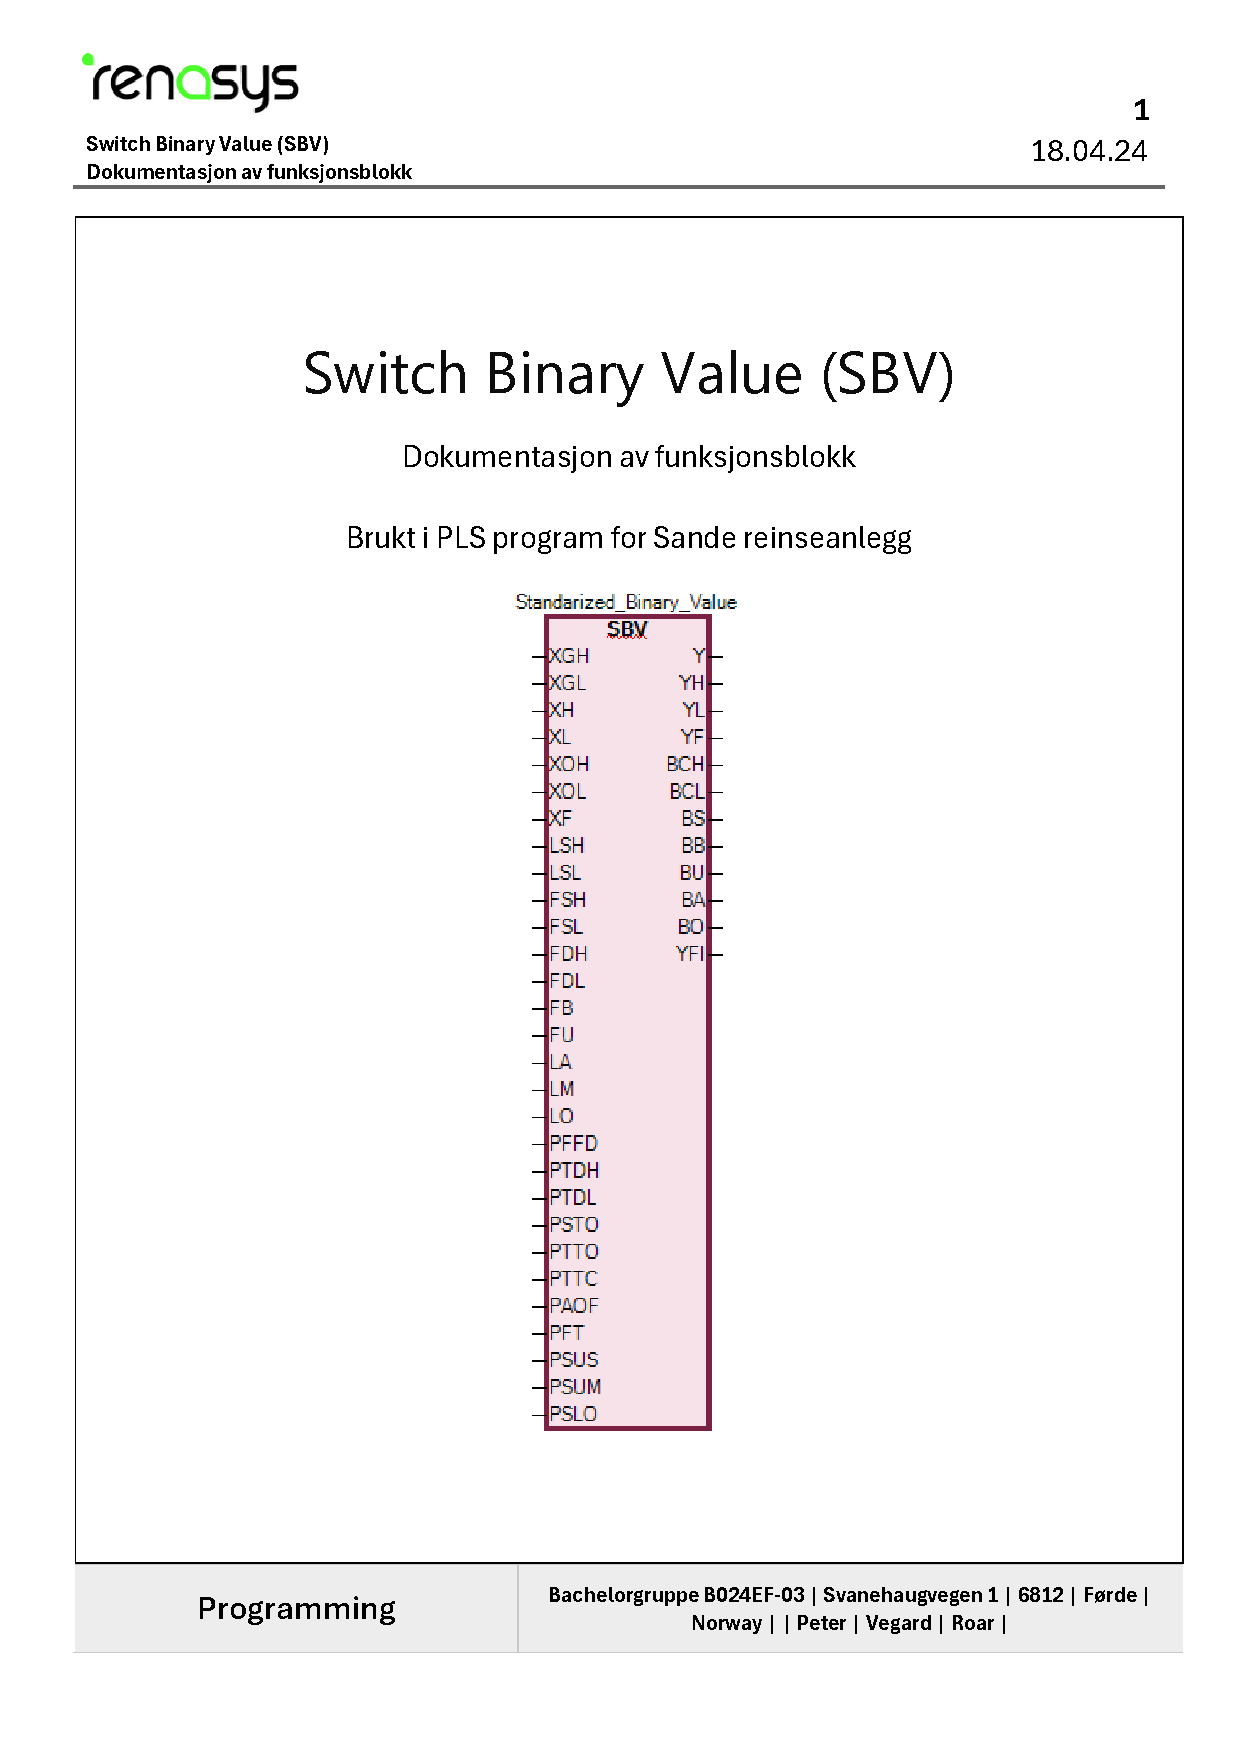
\includepdf[pages=1, scale=0.8, pagecommand={\section{Switch Binary Value}\thispagestyle{empty}}, fitpaper=true ]{Appendix/IEC Blokker/SBV Dokumentasjon.pdf}
\includepdf[pages=2-,scale=0.8, pagecommand={\thispagestyle{empty}},fitpaper=true]{Appendix/IEC Blokker/SBV Dokumentasjon.pdf}

% Litt enklere format
%\includepdf[pages=-, pagecommand={\thispagestyle{empty}}]{Appendix/IEC Blokker/MB Dokumentasjon.pdf}
%\section{MA Blokk}
%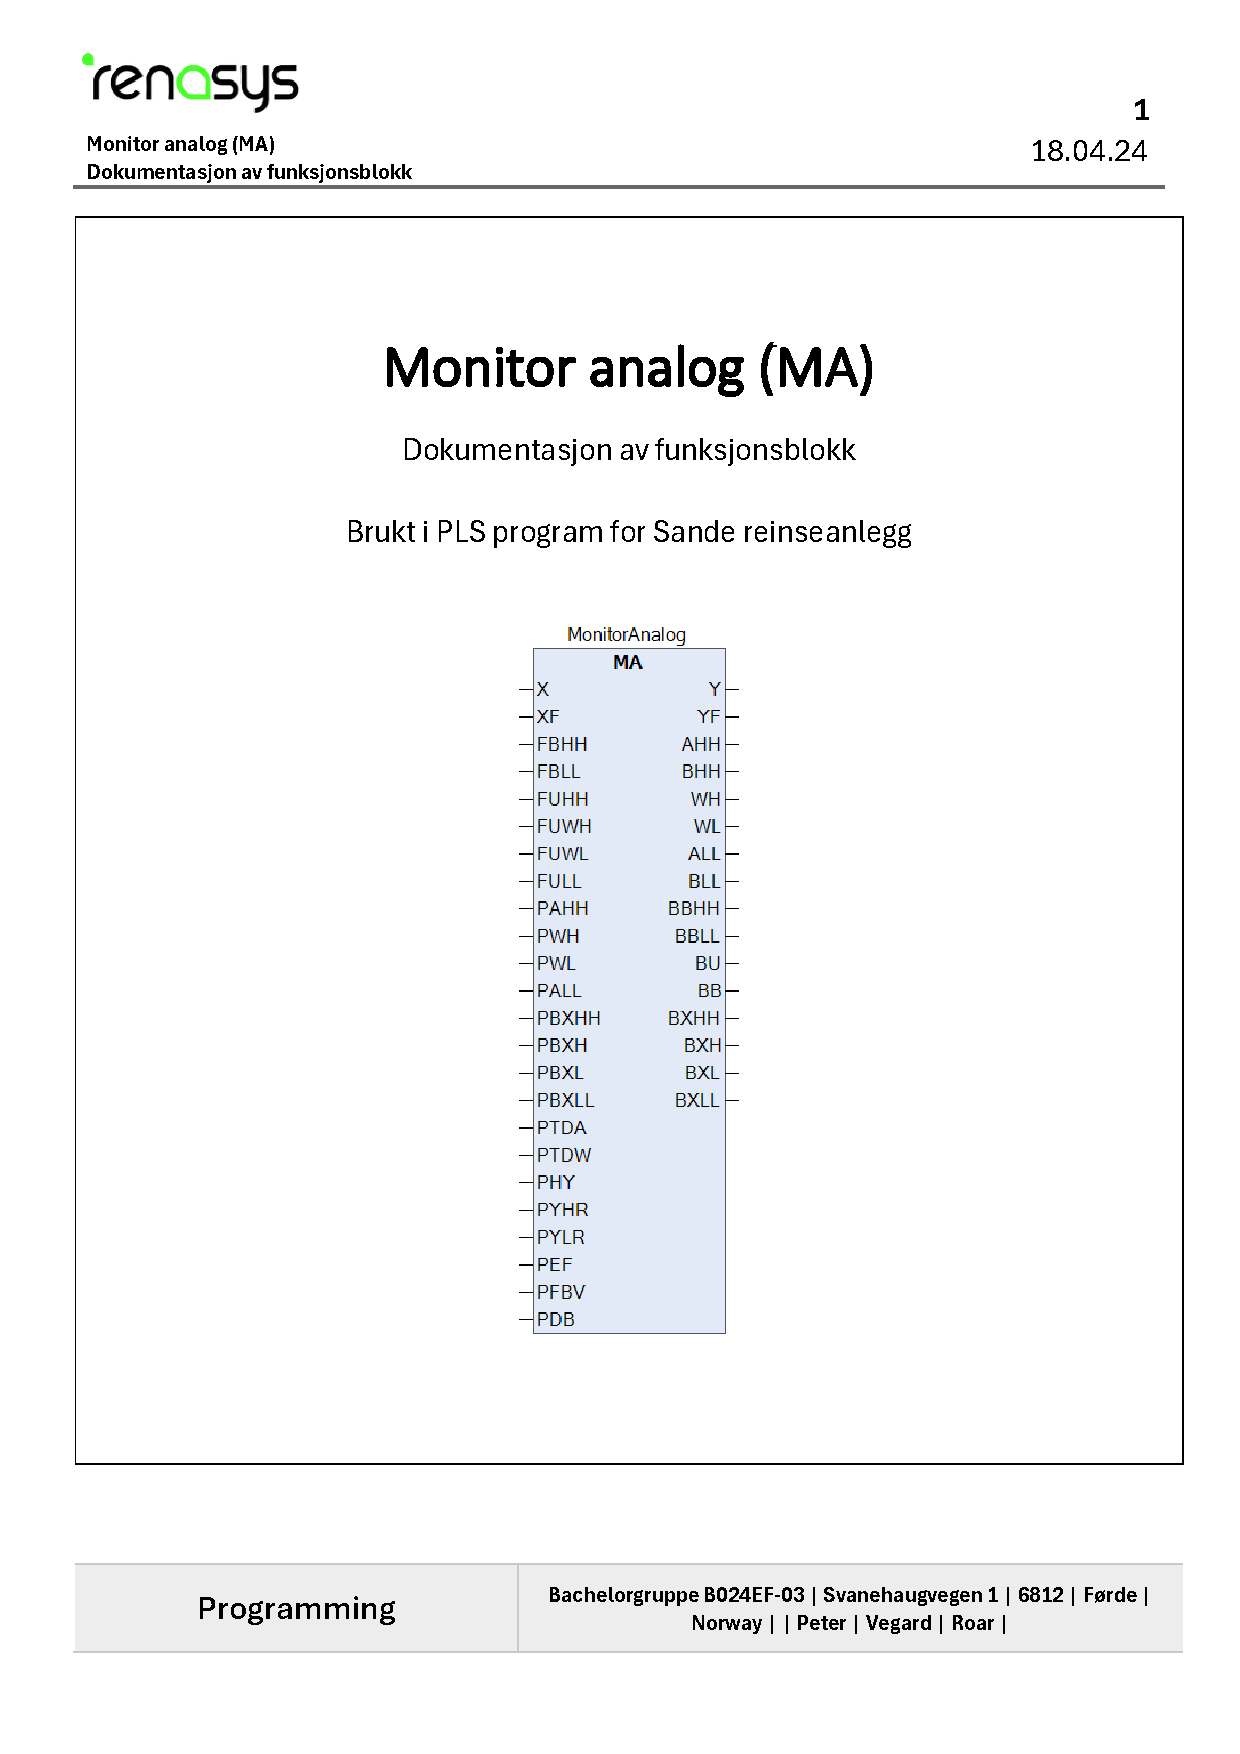
\includepdf[pages=-, pagecommand={\thispagestyle{empty}}]{Appendix/IEC Blokker/MA Dokumentasjon.pdf}
	%	% Stop capturing contents and print them
	%	\stopcontents[appendices]
	%\end{appendices}




	

\end{document} % Dokument slutt


